% **************************************************
% Document Class Definition
% **************************************************

\documentclass[
	paper=A4,
	twoside=true,        % onesite or twoside printing
	openright,           % doublepage cleaning ends up right side
	parskip=full,        % spacing value / method for paragraphs
	chapterprefix=true,  % prefix for chapter marks
	11pt,                % font size
	headings=normal,     % size of headings
	bibliography=totoc,  % include bib in toc
	listof=totoc,        % include listof entries in toc
	titlepage=on,        % own page for each title page
	captions=tableabove, % display table captions above the float env
	draft=false,         % value for draft version
]{scrreprt}


% **************************************************
% Information and Commands for Reuse
% **************************************************

\newcommand{\thesisTitle}{Form and Content in Neural Networks}
\newcommand{\thesisName}{Alejandro Avil\'es}
\newcommand{\thesisSubject}{Unconventional Applications of Deep Learning}
\newcommand{\thesisDate}{September 6, 2016}
\newcommand{\thesisVersion}{0.3}
\newcommand{\thesisFirstSupervisor}{Fernando Berzal}
\newcommand{\thesisUniversity}{\protect{University of Granada}}
\newcommand{\thesisUniversityDepartment}{Department of Computer Science and Artificial Intelligence}
\newcommand{\thesisUniversityInstitute}{International School for Postgraduate Studies}
\newcommand{\thesisUniversityGroup}{Master in Soft Computing and Intelligent Systems}
\newcommand{\thesisUniversityCity}{Granada}
\newcommand{\thesisUniversityCountry}{Spain}
\newcommand{\thesisUniversityStreetAddress}{Periodista Daniel Saucedo Aranda Street}
\newcommand{\thesisUniversityPostalCode}{18071}


% **************************************************
% Load and Configure Packages
% **************************************************

% -- Base packages -------------------------------------------------------------

\usepackage[utf8]{inputenc}
\usepackage[english]{babel}
\usepackage[
	figuresep=colon,
	sansserif=false,
	hangfigurecaption=false,
	hangsection=true,
	hangsubsection=true,
	colorize=full,
	colortheme=bluemagenta,
	bibsys=biber,
	bibfile=thesis,
	bibstyle=numeric,
]{cleanthesis}


% -- Extra packages ------------------------------------------------------------

\usepackage{amsfonts}
\usepackage{amsmath}
\usepackage{mathtools}
\usepackage{subcaption}
\usepackage{todonotes}

\usepackage{enumitem}
\setlist{noitemsep}


% -- Extra config --------------------------------------------------------------

\hypersetup{
	pdftitle={\thesisTitle},
	pdfsubject={\thesisSubject},
	pdfauthor={\thesisName},
	plainpages=false,
	colorlinks=false,
	pdfborder={0 0 0},
	breaklinks=true,
	bookmarksnumbered=true,
	bookmarksopen=true,
	hypertexnames=true
}


% **************************************************
% Document CONTENT
% **************************************************

\begin{document}

% Rename document parts
\renewcaptionname{english}{\figurename}{Fig.}
\renewcaptionname{english}{\tablename}{Tab.}


% -- Front matter --------------------------------------------------------------

% Roman page numbers and no headers/footers
\pagenumbering{roman}
\pagestyle{empty}
% !TEX root = ../thesis.tex
%
% ------------------------------------  --> cover title page
\begin{titlepage}
	\pdfbookmark[0]{Cover}{Cover}
	\flushright
	\hfill
	\vfill
	{\LARGE\thesisTitle \par}
	\rule[5pt]{\textwidth}{.4pt} \par
	{\Large\thesisName}
	\vfill
	\textit{\large\thesisDate} \\
	Version: \thesisVersion
\end{titlepage}


% ------------------------------------  --> main title page
\begin{titlepage}
	\pdfbookmark[0]{Titlepage}{Titlepage}
	\tgherosfont
	\centering

	
\includegraphics[width=5cm]{gfx/logo.png} \\[4mm]
	{\Large \thesisUniversity} \\[4mm]
	\textsf{\thesisUniversityInstitute} \\
	\textsf{\thesisUniversityDepartment} \\
	\textsf{\thesisUniversityGroup} \\

	\vfill
	{\large \thesisSubject} \\[5mm]
	{\LARGE \color{ctcolortitle}\textbf{\thesisTitle} \\[10mm]}
	{\Large \thesisName} \\[5mm]

	\vfill
	% \begin{minipage}[t]{.27\textwidth}
	% 	\raggedleft
	% 	\textit{1. Reviewer}
	% \end{minipage}
	% \hspace*{15pt}
	% \begin{minipage}[t]{.65\textwidth}
	% 	{\Large \thesisFirstReviewer} \\
	%   	{\small \thesisFirstReviewerDepartment} \\[-1mm]
	% 	{\small \thesisFirstReviewerUniversity}
	% \end{minipage} \\[5mm]
	% \begin{minipage}[t]{.27\textwidth}
	% 	\raggedleft
	% 	\textit{2. Reviewer}
	% \end{minipage}
	% \hspace*{15pt}
	% \begin{minipage}[t]{.65\textwidth}
	% 	{\Large \thesisSecondReviewer} \\
	%   	{\small \thesisSecondReviewerDepartment} \\[-1mm]
	% 	{\small \thesisSecondReviewerUniversity}
	% \end{minipage} \\[10mm]
	% \begin{minipage}[t]{.27\textwidth}
	% 	\raggedleft
	% 	\textit{Supervisor}
	% \end{minipage}
	% \hspace*{15pt}
	% \begin{minipage}[t]{.65\textwidth}
	% 	\thesisFirstSupervisor\
	% \end{minipage} \\[10mm]

	M.Sc. thesis supervised by \\
	\thesisFirstSupervisor \\[4mm]

	\thesisDate \\

\end{titlepage}


% ------------------------------------  --> lower title back for single page layout
\hfill
\vfill
{
	\small
	\textbf{\thesisName} \\
	\textit{\thesisTitle} \\
	\thesisSubject, \thesisDate \\
	% Reviewers: \thesisFirstReviewer\ and \thesisSecondReviewer \\
	Supervisor: \thesisFirstSupervisor \\[1.5em]
	\textbf{\thesisUniversity} \\
	\textit{\thesisUniversityGroup} \\
	\thesisUniversityDepartment \\
	\thesisUniversityInstitute \\
	\thesisUniversityStreetAddress \\
	\thesisUniversityPostalCode, \thesisUniversityCity\ (\thesisUniversityCountry)
}

\cleardoublepage

% Just page numbers
\pagestyle{plain}
% !TEX root = ../thesis.tex

\pdfbookmark[0]{Abstract}{Abstract}
\chapter*{Abstract}
\label{sec:abstract}

\vspace*{-10mm}
\todo[inline]{Update with final abstract}
This research aims to review unconventional applications of deep learning, focusing on the separation of style and content of images using convolutional neural networks as research is starting to pay attention to this task.
First, in order to have an appropriate context for the discussion, the work will give an introduction to common terms, techniques, and recent breakthroughs in the field of Deep Learning at large and tasks of image recognition in particular.
From then on, it will present how already trained neural networks have been altered and reused for purposes different from what they were initially designed for.

\vspace*{20mm}

{\usekomafont{chapter}Abstract (Spanish)}\label{sec:abstract-diff} \\

\todo[inline]{Translate final abstract to Spanish}

\cleardoublepage

% !TEX root = ../thesis.tex

\pdfbookmark[0]{Acknowledgments}{Acknowledgments}
\chapter*{Acknowledgments 
\includegraphics[scale=0.1]{gfx/determination}}
\vspace*{-10mm}

Firstly, I would like to manifest my sincere gratitude to my supervisor Fernando Berzal for his stellar guidance.
He accepted supervising this thesis in spite of me living abroad and provided me with enough material and inspiration to engage in researching from the very beginning.
He always replied promptly and concisely to my questions and was thorough, honest, and constructive in his criticism, which motivated me greatly to give my 100\%.
Thanks to him, I not only achieved my goals, but I believe I also learned a valuable lesson for my scientific career.
I can only say, without any doubt, it has been for me truly an honor working together.

I must thank my boss Pedro Ferreira at my full-time job for never objecting with accommodating my schedule so that I could spend energy writing this thesis.
Without his understanding and kindness, it would have been impossible to finish in a timely fashion.

I would also like to thank Andrea Santamaría, ever keeping me from feeling \emph{lost} in my journey and making sure I stay well-fed with the food she let me steal from her.
She helped me as well with the trickiest bits of \LaTeX, polishing the introduction chapter, and suggesting ways to organize the bibliography.

Moreover, I extend my acknowledgment to David Medina, finishing his thesis too, for being a restless companion along these months, and to Mohanty Sharada, for his thought-provoking discussions about Deep Learning.

Last but not the least, I am also grateful to my mother, sister, and friends, who supported me throughout the duration of my efforts.
I wish I could have been there for them much more than I managed to.

Some final words of appreciation to a few of the many other little things.
To Undertale, whose story filled me with \emph{determination}.
To Headspace, whose daily teachings reminded me to stay sharp even in moments of stress.
To all the fantastic music that accompanied me during countless hours of solitary writing, which helped me forget about the time passing.
Moreover, to the rainy, rather chilly summer in good old Geneva, without which staying indoors, working on this thesis, would have posed a much more arduous task.

\cleardoublepage

\setcounter{tocdepth}{2}
\tableofcontents
\cleardoublepage


% -- Body matter ---------------------------------------------------------------

% Arabic page numbers and fancy header/footer
\pagenumbering{arabic}
\setcounter{page}{1}
\pagestyle{maincontentstyle}

% !TEX root = ../thesis.tex

\chapter{Introduction}
\label{sec:intro}

\cleanchapterquote{Computers are useless. They can only give you answers.}{Pablo Picasso}{}

In recent years the field of Deep Learning has experienced a quick growth. As techniques, hardware, and big volume of data, necessary to train deep Artificial Neural Networks (ANN) became a commodity performance of these sky-rocketed and we have seen problems being approached from the perspective of machine learning that no one before could have imagined.

% We will focus on one of these problems. The separation of style and content in images.

% While a human can easily tell when a piece of art is done in a similar style of another, the perception required


% ------------------------------------------------------------------------------

\section{Problem Statement an Motivation}
\label{sec:intro:motivation}

\todo[inline]{Explain why separation of style and content is difficult and what is unconventional about how the task is being approached}


% ------------------------------------------------------------------------------

\section{Goals}
\label{sec:intro:goals}

Artificial Neural Networks in general and Deep Learning in particular are extensive fields that find themselves in constant revision in current times and one could easily fall down the rabbit hole of history, generalities, cutting edge methods or technical details. In an effort to limit how deep we run into and to stay in topic, the scope of this supervised research project has been restricted to the following goals:

\begin{enumerate}
  \item Finding unconventional applications for Deep Learning.
  \item Study separation of style and content
  \item Explore implications patterns neural networks learn and can be exploited for different uses.
\end{enumerate}


% ------------------------------------------------------------------------------

% \section{Results}
% \label{sec:intro:results}
%
% \todo[inline]{If I end up implementing something, present results here}
%
% \subsection{Some References}
% \label{sec:intro:results:refs}
% \cite{WEB:GNU:GPL:2010,WEB:Miede:2011}


% ------------------------------------------------------------------------------

\section{Thesis Structure}
\label{sec:intro:structure}

\textbf{Chapter \ref{sec:related}} \\[0.2em]
In chapter \ref{sec:related} I introduce and discuss the results presented by \cite{Gatys2015}, work which inspired this research project. I present as well prior and derived works that further outline the task of separating style and content on images.

\textbf{Chapter \ref{sec:concepts}} \\[0.2em]
In chapter \ref{sec:concepts} I will briefly go over common concepts needed to understand both the underlaying workings of the different approaches to separation of style and content.

\textbf{Chapter \ref{sec:system}} \\[0.2em]
In chapter \ref{sec:system} I will explain how separation of style and content is tackled in an unconventional way. Instead of training a NN, an already trained one is used and tweaked to perform the operation.

\textbf{Chapter \ref{sec:conclusion}} \\[0.2em]
Finally, in chapter \ref{sec:conclusion} I will muse about the implications of NN being able to extrapolate their past experience to tackle problems for which they weren't trained for.

% !TEX root = ../thesis.tex

\chapter{Theory}
\label{chap:theory}

\cleanchapterquote{At the end of the century one will be able to speak of machines thinking without expecting to be contradicted.}{Alan Turing}{(Computing Machinery and Intelligence in 1950)}


% ------------------------------------------------------------------------------

In this chapter, I cover the basic concepts of neural networks that will be used later on when separation of style and content is discussed in more detail.
My intention is to allow anybody with basic knowledge in Mathematics and Computing to understand this manuscript from beginning to end.

The explanations will be developed from basic to complex so that sequential reading should guide the reader logically from question to answer while giving as much insight as will be necessary to continue and just enough context to understand the raison d'être of the each concept.


% ------------------------------------------------------------------------------

\section{Background}
\label{sec:theory:background}

Before diving into technical aspects, however, I believe it is worth stopping first to introduce the main areas of this research: \emph{Neural Networks} and \emph{Deep Learning}.
Neural Networks is an area of \emph{Machine Learning} very closely related with \emph{Cognitive Sciences} and Deep Learning is also an area of Machine Learning that typically uses neural networks, but let us go step by step.


\subsection{Neural Networks}
\label{sub:theory:background:neural-networks}

We can describe the field of Machine Learning as the study that enables computers to resolve problems for which they have not been explicitly programmed for by using some learning mechanism, as \citet{Samuel1959} postulated.
When explicitly programming an algorithm to resolve a problem, its complexity grows dramatically with that of the problem and the desired precision.
A perfectly robust algorithm that follows this approach will require: 1) the programmer to understand the problem completely so that all variables can be taken into account; 2) a hardware powerful enough to handle all these variables; and 3) data with maximum precision.
It is easy to see how one or more of these requirements will pose complications when the problem is complex enough.
Driving a car is a complex enough problem to make classic computing incapable of solving it.
Conversely, driving a car is a simple enough problem so that any person can do it.
The human mind can handle the task because, although not having perfect senses nor 100\% understanding of the laws of physics, how the car works, how other drivers exactly behave, and many other factors involved; it is capable of dealing with partial information, uncertainty, imprecision, and approximations after having learned from experience \cite{Zadeh1994}.
In contrast to how classic computing tries to accurately model the world to solve problems, some fields of Machine Learning try to model how the human mind learns the complexity of the world to reason and act upon it.

At this point, it is clear how the study of the human mind plays an important role in machine learning.
Cognitive sciences is the field that studies the human mind and how it acquires understanding through experience and the senses.
Modern cognitive sciences originated in the 1940s, when efforts were being made to understand the principles of the mind by representing their structures and processes instead of operating directly on them \cite{Thagard2008}.
The studies quickly branched off in 1943 when \citet{McCulloch1943}, inspired by biological neural networks, described the first mathematical model of an artificial neural network.
The field of Neural Networks, shorthand for \emph{Artificial Neural Networks} (ANNs), quickly grew in the 1950s when they started being implemented \cite{Farley1954,Rosenblatt1958}.

Since then, the field has evolved and expanded into a myriad of different methods, maintaining the similarity with their biological counterparts in greater or lesser degree.
Within the general framework, we can still talk of neurons organized in \emph{layers}, implementing an \emph{activation function}, and storing experience in \emph{weights}, as depicted in Figure~\ref{fig:sec:theory:neurons}.
An artificial neuron is a simple processing unit, forming networks typically organized in layers, whose input is the set of outputs of connected neurons from the previous layer and where the process it performs is determined by the activation function.
The activation function can be implemented either as a threshold to be reached for the neuron to send an output or simply as a transformation of any sort of the input.
Lastly, experience in ANNs can be understood as connection strength between neurons in biological neural networks and this mechanism is implemented as a set of learnable parameters, commonly called weights, that modify the value of each input to the neuron \cite{Hinton1989}.

\begin{figure}[t]
  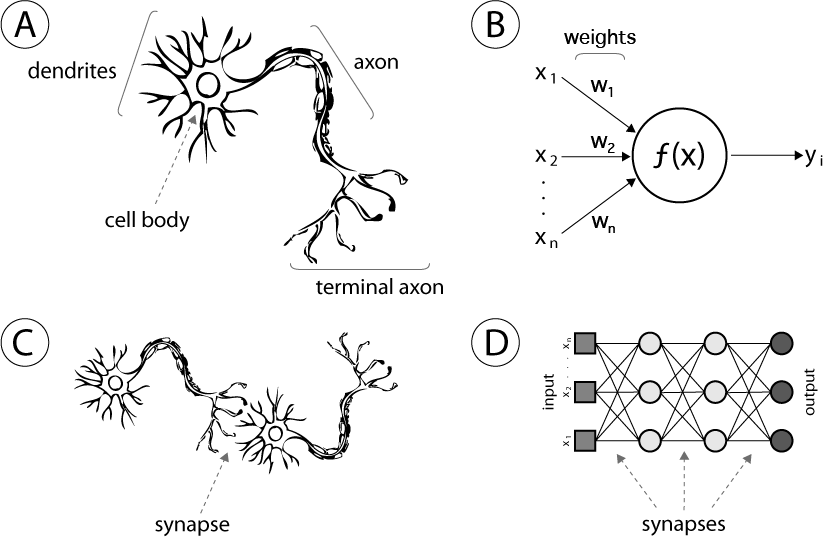
\includegraphics[width=\textwidth]{gfx/neurons}
  \caption{
    Biological Neuron vs. Artificial Neuron \cite{Honorio2013}.
    AC) A biological neuron receives signals at the dendrites, the composition of the signals may or may not produce an excitation in the cell body based on experience, in which case a pulse will be transmitted down the axon and ultimately to other neurons' dendrites via terminal axon in a process called synapsis.
    BD) Similarly, artificial neuronal networks are organized in layers and synapses occur from layer to layer.
    An artificial neuron in the layer $Y$ receives one or more inputs $X$, representing dendrites, and as a result of an activation function $f(X)$ produces an output $y_i$, representing the axon, that gets passed to connected neurons in the subsequent layer.
    Weights represent the connection strength between neurons and encode network experience.
  }
  \label{fig:sec:theory:neurons}
\end{figure}

A crucial step in preparing an ANN for a specific task is refining its set of weights.
That is what we refer to as training or supervised learning process.
Supervised learning is a data-driven process that requires a labeled training set of examples of which we know their class (e.g. dog vs. cat).
The process can be implemented in several ways but it generally boils down to defining some way to assess how far the prediction of the network is away from an optimal solution, an estimate given by a \emph{loss function}, and the strategy that will propagate the error as well as refine the weights of the network.
Eventually, after enough training examples and corrections, the weights of the network will have adapted to generalize the features of the training data and will be more or less able to correctly classify new incoming examples.

The process can be seen as a teacher supervising the learning of a student.
The ``teacher" (loss function + weight rectification strategy) knows the correct solution (label of the example) and it corrects the ``student" (the network) when its prediction is incorrect.
An example of a completely wrong prediction would be the network having 100\% confidence of an image containing a dog when it clearly contains a cat.

One of the most important aspects that determine the accuracy of the network when presented with new examples is the volume of data and the correctness of its labels.
This becomes extremely important when trying to solve real-world problems like image recognition, where massive training sets are required to generalize networks for all concepts in a language under several different lighting conditions.
Big enough volumes of data have not been readily available until recently, and even nowadays, complete and accurately labeled datasets are expensive or time consuming to handcraft as the task may be too large or require expert knowledge on the specific field.
One approach to work around this is semi-supervised learning, using partially labeled training datasets and pre-training the network first with unsupervised training, where unlabeled examples are employed so that the network learns how to identify recurring patterns, which are later employed to improve the performance of the supervised learning process \cite{Zhu2008}.
Reducing the number of weights the network requires to correctly classify the input is another complementary solution that has seen much success lately and it is one of the recurring features of many deep learning techniques.


\subsection{Deep Learning}
\label{sub:theory:background:deep-learning}

Since 2006, the field of \emph{Deep Learning}, also called hierarchical learning, has appeared as a new area of Machine Learning research that brings it closer to its original goals: Artificial Intelligence \cite{Deng2014}.
Deep learning focuses its efforts on producing methods for learning hierarchical feature representations, different levels of abstraction where higher-level ones are defined from lower-level ones, helping to make sense of data such as images, sound, and text in real-world applications.

One clear example of hierarchical representation is a spoken sentence.
A spoken sentence, the higher-level concept, is composed of spoken words.
A spoken word is made up of phonemes.
A phoneme is a representation of a speech sound with an associated waveform.
Making sense of speech in deep learning means first analyzing the waveform looking for phonemes, then trying to make up words from the phonemes found, and finally producing a grammatically correct and semantically meaningful sentence with those words.

As already mentioned in Chapter~\ref{chap:intro}, this kind of pattern recognition did not perform well until recently.
Traditional solutions employed shallow neural networks with simplistic models and limited representation power that could only be used to solve well-constrained problems like numerical approximations or binary classification.
Speech recognition, contrarily, is a very loosely-constrained problem and that is also the case for any problem dealing with the richness of data such as human voice, natural language, and natural images.

Studies in human information processing mechanisms suggested the human brain uses deep neuronal architectures to extract complex patterns and build internal representations from rich sensory inputs.
For instance, the human speech perception system in the brain is equipped with layered hierarchical structures that transform the information from the acoustic level to the linguistic level \cite{Deng1999,Baker2009}.
Training analogous deep architectures in artificial neural networks, \emph{deep neural networks} (DNNs), proved problematic from the beginning since classic learning algorithms tended to quickly get stuck in local optima and produced inaccurate classifications.
This phenomenon, unfortunately, worsened quickly the more layers the neural network presented, which is the case of DNNs.

Efficient unsupervised learning algorithms that made use of increasingly big datasets, available thanks to the widespread use of the Internet, were proposed to overcome the problems presented by local optima in classic learning algorithms \cite{Bottou2004,Hinton2006}, as previously discussed in Section~\ref{sub:theory:background:neural-networks}.
They, however, were so computationally expensive for training deep neural networks, having millions of parameters to learn, that were not widely used until parallelizable variations were proposed \cite{Dean2012,Chen2012}.
Powerful Graphic Processing Units (GPUs) becoming a commodity finally allowed quick implementations of these algorithms and marked the rapid development of deep learning in recent years.

Deep Learning is at the moment a quickly growing field covering a wide range of machine learning techniques and architectures.
In this research, we cover only the architecture of DNNs that we need for further discussing the separation of style and content, \emph{convolutional neural networks} in Section~\ref{sec:theory:convnets}.
Before jumping too far ahead, the next sections of this chapter will go through the evolution of relevant ANNs architectures down from the most basic one, the \emph{perceptron}, up to the one at hand, convolutional neural networks.


% ------------------------------------------------------------------------------

\section{Perceptron}
\label{sec:theory:perceptron}

The perceptron was the first ever implemented neural network.
It was created by \citet{Rosenblatt1958} in 1957 based on the studies of \citet{McCulloch1943} and it featured the simplest architecture possible in an ANN, composed of a single neuron.

The perceptron can be described as performing a task of binary classification, which is simply deciding which of two mutually exclusive classes a set of inputs belongs to \cite{Freund1999} and it is mathematically expressed as follows:

$$
  f(x) =
  \begin{cases}
    1 & \text{if } {w}\cdot{x}+b > 0\\
    0 & \text{otherwise}
  \end{cases}
$$

Where $x$, an array of real values, represents the input of the perceptron; $w$, also an array of real values, represents the weights; $b$ is the \emph{bias}; ${w}\cdot{x}$ is the dot product; ${w}\cdot{x}+b > 0$ is the activation function; and, finally, $0$ and $1$ correspond to the mutually exclusive classes.

The inputs are visualized as data points in the space of variables and the activation function as a linear boundary that leaves them classified either above or below it.
The weights are used to measure the relevance of each one of the inputs in the final classification, parameters that get learned during the training process in the same fashion as I described in Section~\ref{sub:theory:background:neural-networks}.
The bias gets also learned during the training process, but it does not depend on any input value and is used to control the position of the linear boundary.
The dot product can also be expressed as a weighted sum $\sum_{i=0}^{m} w_i x_i$ where $m$ is the number of parameters the perceptron receives per input, as it is depicted in Figure~\ref{fig:sec:theory:perceptron}.

\begin{figure}[t]
  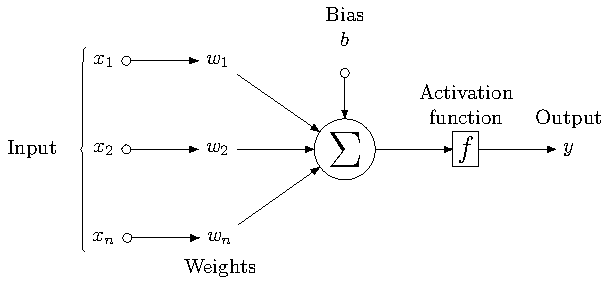
\includegraphics[width=\textwidth]{tkz/perceptron}
  \caption{
    Anatomy of the Perceptron \cite{Medina2013}.
    In the center, represented by $\sum$, there is the weighted sum of inputs.
    Mathematically expressed as the dot product (${w}\cdot{x}$) of the vector of inputs $x$ with the vector of weights $w$, both containing real values.
    The activation function triggers a binary output $y$ if ${w}\cdot{x}$ plus the bias $b$, also a real value, is above $0$.
  }
  \label{fig:sec:theory:perceptron}
\end{figure}

Perceptrons can be trained with supervised learning for trying to find the weights in the binary classifier function to correctly classify some training dataset.
Let us imagine we want to train a perceptron to classify animals into either cat or dog based on their size and level of domestication.
Our training data is labeled, meaning that for each pair $(size, domestication)$ we know whom it actually belongs to, either a cat or a dog.
We start with a perceptron whose weights are set to random values and the first training example gets classified randomly.
As new training examples arrive, the learning algorithm will update the weights of the perceptron so that the linear boundary described by ${w}\cdot{x}+b$, the activation function, leaves data points correctly classified in both sides.
Figure~\ref{fig:sec:theory:perceptron-training} depicts how this process happens.

\begin{figure}[t]
  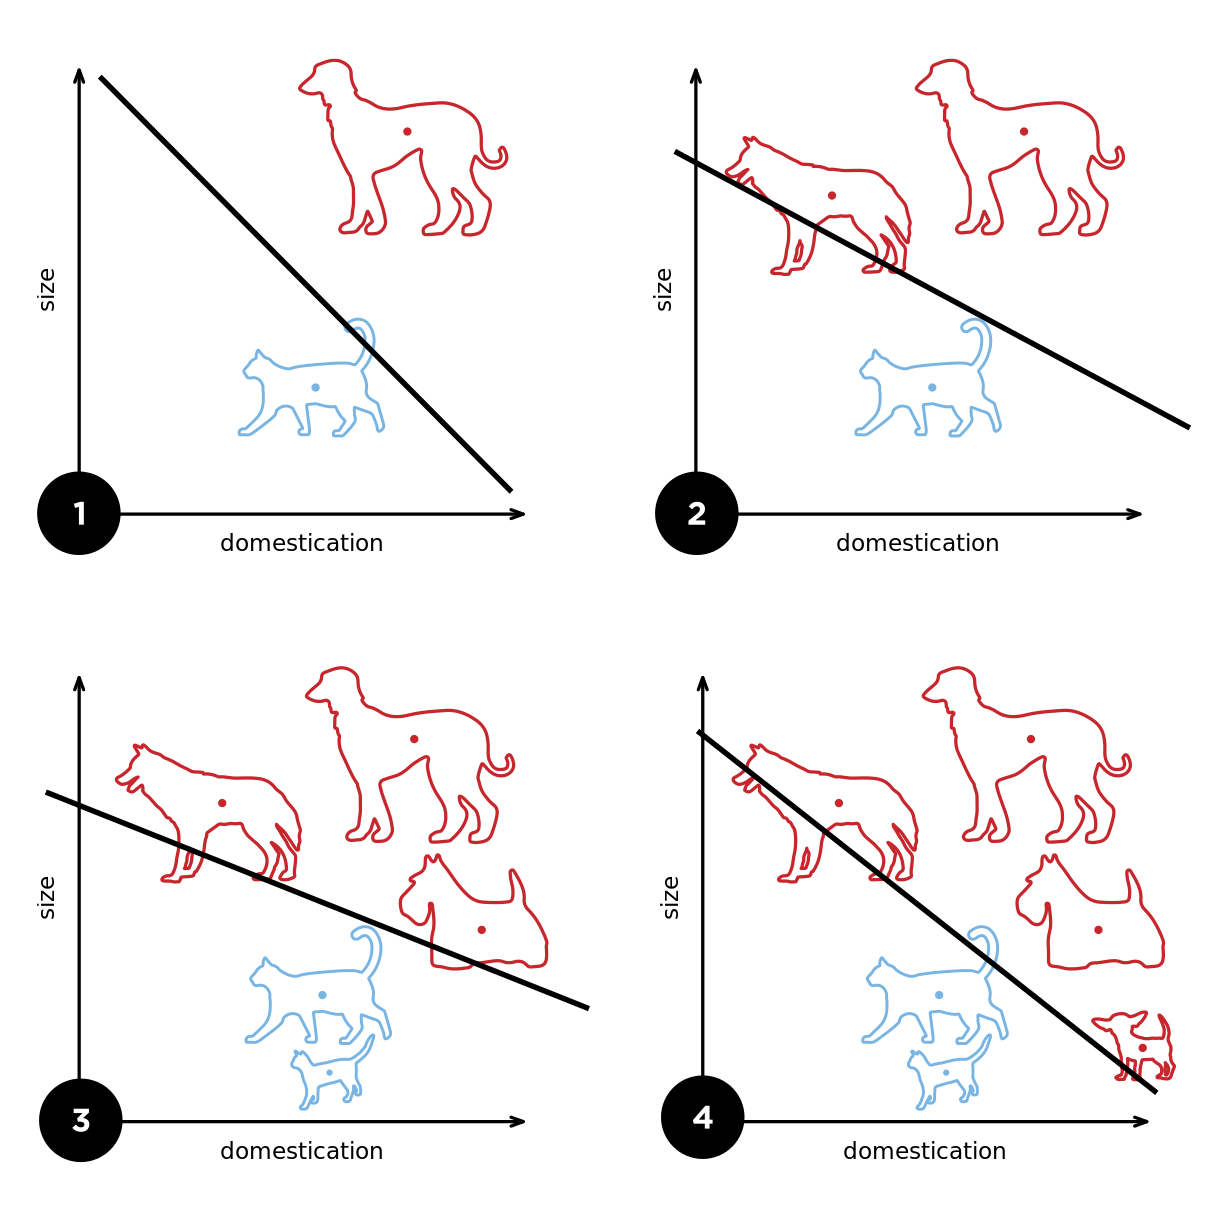
\includegraphics[width=\textwidth]{gfx/perceptron-training}
  \caption{
    Linear boundary of a perceptron adjusting to new training examples \cite{Goodspeed2015}.
    The perceptron classifies inputs with two variables: $size$ and $domestication$, into two classes, dog or cat.
    Supervised learning adjusts the linear boundary to accommodate the new data points into their correct category.
  }
  \label{fig:sec:theory:perceptron-training}
\end{figure}

The main problem with the perceptron is that the training will never converge to a set of weights that correctly classify the training examples if these are not linearly separable, and thus predictions of new data points will consistently be wrong.
These limitations were mathematically proved by \citet{Minsky1969} in 1969.
Not only that, they also claimed perceptrons with multiple layers of neurons would not be capable of overcoming non-linearities, leading to believe that neural networks would not be feasible for scalable intelligent systems and managing to discourage further efforts in the field for over a decade.
Little to none research was done in the field until \emph{backpropagation}, a learning algorithm for \emph{multi-layer neural networks}, was developed by \citet{Werbos1974}, rediscovered by \citet{Parker1985}, and finally popularized by \citet{Rumelhart1986} in the 1980s \cite{Ruck1990}.
The efficient use of multi-layer feedforward neural networks marked the rise in popularity of the field.


% ------------------------------------------------------------------------------

\section{Multi-layer Feedforward Neural Networks}
\label{sec:theory:mlffnn}

While introducing the perceptron, we could not really speak of it as neural network per se, since we were discussing an architecture consisting of a single neuron.
We introduce now multi-layer feedforward neural networks, composed of several layers of neurons, them being fully connected with the neurons of the adjacent layers and data always flowing forward.
Figure~\ref{fig:sec:theory:mlffnn} depicts such \emph{feed-forward} architecture where data flows, represented as arrows, never forms a cycle, opposed to other more complicated types of architectures where data is fed back to previous layers.
These networks behave like we described when talking about the perceptron both in their first layer, representing the parameters of the input, and in their final layer, performing classification.
Intermediate layers, called \emph{hidden layers}, are the most interesting addition to the architecture.
Neurons in them perform intermediate predictions and these are fed to neurons in the next layer.
The fully-connected architecture architecture allows for different neurons in the hidden layers to make predictions of different patterns in the raw input and letting neurons in subsequent layers predict based on those patterns instead.

If we zoomed in on one the nodes we would see replicated exactly the same structure as we presented previously for the perceptron in \autoref{fig:sec:theory:perceptron}.
Inputs get weighted and summed, and the result of that passed to some function that performs the prediction.
One important difference to note is that for the input of subsequent layers to still be real values, neurons in hidden layers must implement non-linear activation functions, representing the probability or certainty of the example belonging to a class.
Non-linear activation functions are also normally called \emph{transformation functions} since they transform the input rather than producing a binary classification.
Non-linearities often used are the hyperbolic tangent, $\tanh(x)$, or the logistic function, $(1+e^{-x})^{-1}$, which are inspired by biological neurons' \emph{action potential}, and allow for non-linear classification \cite{Thorpe1989}.

Unlike the perceptron and contrary to incorrect beliefs induced by a misinterpretation of \citeauthor{Minsky1969}'s analysis of the perceptron limitations, disproved by \citet{Hornik1989} in 1989, multi-layer feedforward networks with at least one hidden layer are capable of making predictions of arbitrary precision given enough data regardless of it being non-linearly separable.
These networks' capabilities make of them universal approximators and viable for intelligent systems, being the key for such an achievement backpropagation, a general purpose supervised learning algorithm for feed-forward networks \cite{Rumelhart1986}.

\begin{figure}[t]
  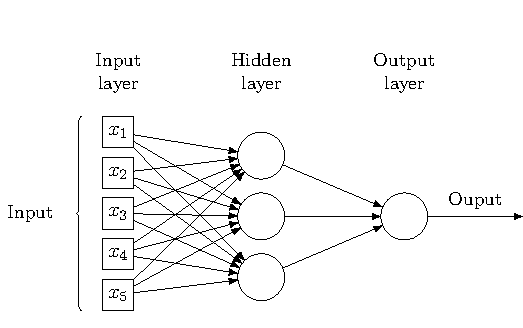
\includegraphics[width=\textwidth]{tkz/mlffnn}
  \caption{
    Architecture of the most simple multi-layer neural network \cite{Medina2013A}.
    The first layer, at the left, represents the parameters of the input that get fed into each one of the neurons of the next layer.
    The last layer, at the right, performs the final classification.
    The layers in between, called hidden layers, also perform intermediate classification and their output is fed as input to the next layer.
  }
  \label{fig:sec:theory:mlffnn}
\end{figure}


\subsection{Backpropagation}
\label{sec:theory:mlffnn:backpropagation}

Training single-layer networks, where the input is directly connected to the output layer, is relatively simple.
As we described before, it only requires iteratively adjusting the weights to correctly classify the training examples based solely on the input parameters.
Training multi-layered networks becomes much more difficult since the final prediction is not directly related to the original input parameters, but to all intermediate predictions in hidden layers and thus to their weights as well.
Consequently, a learning procedure for these networks should determine the weights of neurons in hidden layers that will result in the intermediate predictions that will produce correct predictions at the output of the network.
This is equivalent to making the neurons in hidden layers learn internal representations of incoming data, which is one of the main interests of using multi-layered networks to solve real-world problems that are hard to model, be it due to lack of knowledge in the domain or to the complexity of the task.

Learning in neural networks can be generally approached as an optimization problem.
For each training example $(x, t)$, being $x$ the array of input parameters, we first must find the minima in the error function, e.g. $E = (t - y)^2$, being $t$ the correct prediction, also referred to \emph{ground truth}, and $y$ the prediction of the network.
At the same time, $y$ is a function representing the operation performed by the network as a whole, depending on the weights $w$ that will ultimately be adjusted to minimize the error $E$.

\autoref{fig:sec:theory:mlffnn:error-function} shows the visual representation of the error function for a single-layer neural network with 2-parameter inputs, being $y = w_1 x_1 + w_2 x_2$, the transformation function.
There are several methods to find the minima of such parabolic function, but \emph{gradient descent} is normally used.
In multi-layered networks, on the other hand, $y$ is a composite function of increasingly nested transformation functions on each layer.
For a network, $y$ would be $\sum_i w_i f_i(x)$, being $i$ neurons of the last hidden layer, $w_i$ the weight assigned to their output, and $f_i$ their transformation function, described by $\sum_j w_j f_j(x)$, being $j$ neurons of the previous hidden layer.
This continues until the first hidden layer.
Gradient descent can be efficiently applied on this kind of chained functions using the chain rule, as described by \citet{Linnainmaa1976} and implemented in the backpropagation algorithm.

\begin{figure}[t]
  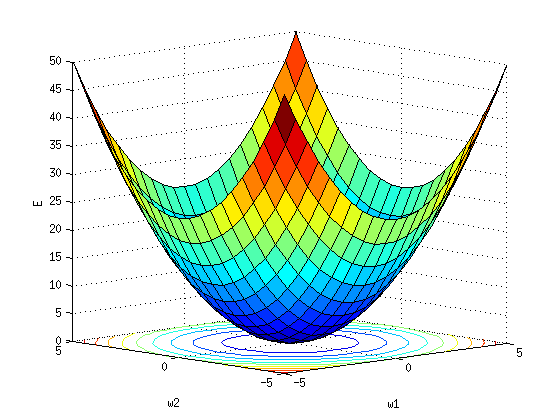
\includegraphics[width=\textwidth]{gfx/error-function}
  \caption{
    Error function of a single-layer neural network with two input weights \cite{AI4562013}.
    The function is defined by $E = (t - (w_1 x_1 + w_2 x_2))^2$ and finds its minima at $E = 0$ when $w_1$ and $w_2$ correctly predict $t$ for the input $x$.
  }
  \label{fig:sec:theory:mlffnn:error-function}
\end{figure}

Backpropagation, inspired on the mathematical intuition, describes an approach for adjusting the weights of the whole network based only on the output prediction error and scales up for arbitrarily big networks by propagating the error and correcting weights locally for each neuron.
The algorithm consists of two phases: 1) error propagation, and 2) weight correction.

During error propagation, for a training example, the algorithm first calculates the error $E$ for the prediction $y$ in the output layer.
The error gets then propagated backwardly to all neurons layer by layer, as represented in \autoref{fig:sec:theory:mlffnn:backprop-1}.
The propagated error for a neuron $i$ within a given hidden layer is calculated as $E_{i} = \sum_j w_{ij} E_{j}$, being $j$ a neuron in the following layer (closer to output), $E_{j}$ its calculated error, and $w_{ij}$ its associated weight for neuron $i$.
Propagated errors represent how much of the overall error was contributed by the neuron on its layer.

\begin{figure}[t]
  \begin{subfigure}[b]{0.5\textwidth}
    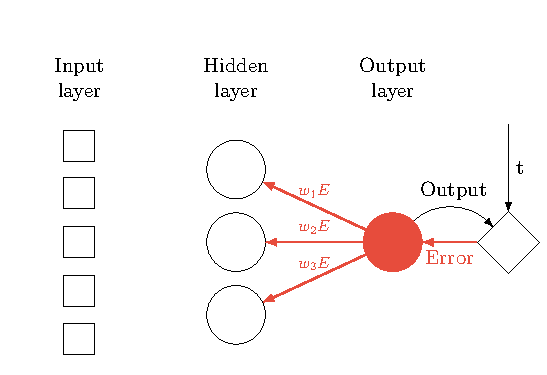
\includegraphics[width=\textwidth]{tkz/mlffnn-backpropagation-1}
    \caption{Error propagation}
    \label{fig:sec:theory:mlffnn:backprop-1}
  \end{subfigure}
  \hfill
  \begin{subfigure}[b]{0.5\textwidth}
    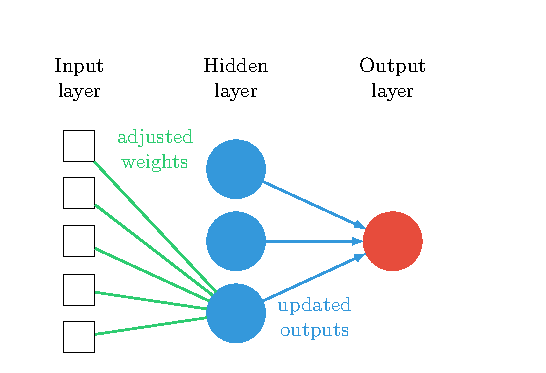
\includegraphics[width=\textwidth]{tkz/mlffnn-backpropagation-2}
    \caption{Weight correction}
    \label{fig:sec:theory:mlffnn:backprop-2}
  \end{subfigure}
  \caption{
    Backpropagation.
    During error propagation (a), the error $E$, calculated as $t - y$, is propagated from the output layer to all hidden layers, representing how much each neuron contributed to the overall error.
    During weight correction (b), now that the contributed error $E_{ij}$ for every neuron is known and starting by the first hidden layer, weights are updated in a neuron by finding the values that minimize said error for the original input received.
    In subsequent layers, new weights are calculated similarly but using the updated outputs from the previous layer instead.
  }
  \label{fig:sec:theory:mlffnn:backprop}
\end{figure}

Once the contributed error has been calculated for the first hidden layer, the weight correction phase begins.
Starting from the first hidden layer, each weight $w_i$ of a neuron is adjusted by finding the optimal value $w'_i$ that minimizes the error $E$ for that neuron, calculated through error propagation, using the original input $x$.
The variation $\Delta w_i$ to be applied on $w_i$ is calculated by finding the partial derivative of the error with respect to $w_i$, which can be analytically calculated \cite{Orr2008} as:

\begin{equation}
  \Delta w_i =
    -\alpha \frac{\partial E}{\partial w_i} =
    -\alpha E f'({w}\cdot{x}) x_i
\end{equation}

Being $f'$ the derivative of the activation function, $\alpha$ the learning rate, carefully picked to make the optimal weights converge, and $-1$ a constant to ensure descent in the algorithm.

Weight correction for neurons in subsequent layers is performed similarly layer by layer until the whole network is updated, the only difference their inputs being the new output $x'$ as a result of neurons in previous layer with their now updated weights $w'$ as depicted in \autoref{fig:sec:theory:mlffnn:backprop-2}.

For a visual step by step explanation of backpropagation, I recommend further reading \url{http://home.agh.edu.pl/~vlsi/AI/backp_t_en/backprop.html} \cite{Bernacki2005}.

There is still one final concern when training fully-connected networks.
Backpropagation teaches networks to predict samples from the training dataset accurately, but the ultimate goal of the training, we must not forget, is making the network capable of predicting unseen samples.
We, therefore, evaluate the performance of a trained network based on how accurate it predicts unseen samples.
One of the main reasons why a network may fail at this is \emph{overfitting}, and fully-connected networks are remarkably prone to suffer it.


\subsection{Overfitting}
\label{sec:theory:mlffnn:overfitting}

We refer to overfitting when a trained neural network has excellent accuracy against samples in the training dataset, but low accuracy against unseen samples.
Overfitting occurs as a result of a dataset not containing enough samples to train the network.

When there are fewer training samples than learnable parameters the network will simply ``memorize'' how to match training samples to correct predictions.
If more training samples are given than $input \mapsto prediction$ associations the network can ``memorize'', it will be forced to learn patterns instead.
For instance, going back to the example of classifying animals as either cat or dog we used in \autoref{sec:theory:perceptron}, if we only had two training samples: a cat, small and wild; and a dog, big and docile; the network would wrongly assume all small animals are cats and a chihuahua would end up classified as a feline.

Dealing with overfitting is not a trivial matter, especially when training big networks for real-world applications.
These kind of applications require networks big enough to learn the complexity of real-world pattern recognition tasks, but big networks require larger datasets and are more sensitive to noisy data and irrelevant information.

Preparation of training datasets for training effective networks becomes crucial, but reducing noise is generally costly and deciding what information is relevant often requires expert knowledge.
On top of it, learnable parameters increase exponentially when the input data is rich or the network has multiple layers, and because of this, vast amounts of training data are required, making the dataset preparation process even more laborious.

Although feedforward networks are universal approximators, their significant amount of learnable parameters architecture makes them extremely prone to overfitting, as they quickly grows with every neuron added to the network.
Overfitting made these networks outperformed by domain specific algorithms, relegating them to a secondary position in many areas of Machine Learning for some time.
In tasks like image or speech recognition, fully-connected networks suffered terribly the effects of overfitting to the point of not being truly usable, displaying frustrating performance when used in end-user applications as I illustrated in Chapter~\ref{chap:intro}.

We will next discuss how convolutional neural networks, developed in the late 90s, eventually proposed a feed-forward multilayer architecture capable of performing robust image and speech recognition, among others tasks.
They require far fewer learnable parameters than their fully-connected counterparts, making them less prone to overfitting, and are currently the state of the art in many pattern recognition tasks.


% ------------------------------------------------------------------------------

\section{Convolutional Neural Networks}
\label{sec:theory:convnets}
Convolutional neural networks, also known as CNNs or ConvNets, are feed-forward multilayer neural networks inspired by cats' and monkeys' visual ventral stream \cite{Hubel1968,Lawrence1997} and are responsible for a major breakthrough in image recognition \cite{LeCun1995}.
Before and contemporaneous to \citeauthor{LeCun1998}'s LeNet \cite{LeCun1998} other networks like \citeauthor{Fukushima1980}'s Neocognitron \cite{Fukushima1980} or \citeauthor{Riesenhuber1999}'s HMAX \cite{Riesenhuber1999} were also inspired in the visual cortex, but it was the former that established the fundamentals for CNNs.
They are able to learn patterns in images from a training set through back-propagation and present built-in resilience towards translation and distortion variances in the input.
Such resilience minimizes pre-processing tasks both for training and classification and greatly reduces human supervision, making CNNs the currently preferred system for image recognition \cite{Visin2015}.

Multi-layer feedforward networks were able to perform image recognition \cite{Zhang1999} but in order to reduce the effects of overfitting they could only perform scope-specific predictions on low-res images that had to be processed beforehand to reduce noise.
Fully-connected layers scale poorly since neurons of the first hidden layer will process the whole image and will need to store weights for every color channel of every pixel.
Just to give a sense of the scale we are talking, for an RGB image of ${N}\times{M}$ pixels, every neuron in a multi-layer feedforward neural network will require storing ${N}\times{M}\times{3}$ weights, which for a ${32}\times{32}$ image it is $3072$ weights, but for a ${1024}\times{1024}$ one is more than $3$ million.
This means a quadratic memory growth $O(N^2)$ with respect to image resolution.
Not only this is the cause of huge overfitting effects, it also implies a performance issue in terms of hardware resources.

One big wrong assumption in conventional feedforward networks is treating each input parameter individually as non-correlated data.
This is false in tasks of signal processing, speech recognition, or image recognition.
For instance, let us image a set of images containing a red apple.
Pixels on it are not randomly distributed but, rather, red-hued pixels are expected to bunch together.
It seems the rule \emph{``bunch of red-hued pixels $\mapsto$ apple''} should be sufficient to recognize an apple, no matter if the bunch of pixels appears either centered or shifted to one side.
The pitfall of fully-connected networks is two-fold here.
On the one hand, the network will probably fail if the apple is shifted too much on one side since it did not just the rule proposed before but more likely: \emph{``pixels in positions $(4, 4)..(4, 6)...(6, 4)..(6, 6)$ are red $\rightarrow$ apple''}.
On the other hand, every neuron ``sees'' the whole image so the rule will be learned in several different sub-networks as some sort of brute-force pattern learning.
This intuition tells us fully-connected networks require a bigger amount of learnable parameters that should be needed and that is, in fact, the cause of overfitting problems.


\subsection{Properties}
\label{sub:concepts:convnets:properties}

CNNs can take advantage of spatial information inherent in data thanks to a number of CNN architectural features \cite{LeCun1998}: 1) local receptive fields, 2) shared weights, and 3) subsampling.

\begin{figure}[t]
  \begin{center}
    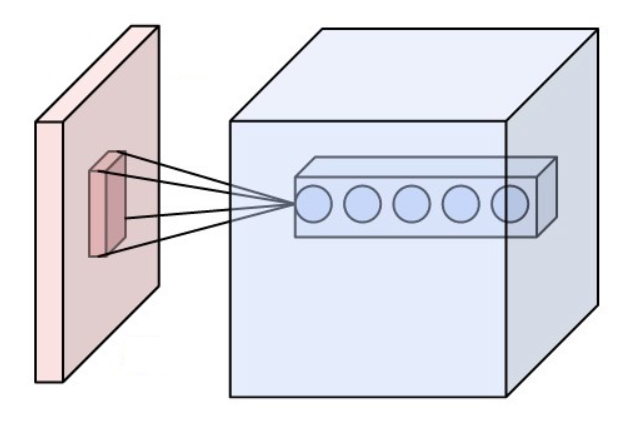
\includegraphics[width=0.6\textwidth]{gfx/conv-layer-1}
  \end{center}
  \caption{
    Stack of neurons applying different feature detections within a convolutional layer on the same perceptual region \cite{Aphex342015}.
  }
  \label{fig:sec:theory:convnets:conv-layer-1}
\end{figure}

\paragraph{Local receptive fields}
The term \emph{receptive field} is borrowed from the literature of neuroscience and it refers to an area of the body surface that triggers a neurological response in the presence of stimuli \cite{Sherrington1906,Alonso2008}.
In the context of convolution networks, receptive field refers to a region of the visual input, represented by an image, that is connected with one or several neurons that will react to it and is commonly called \emph{filter}.
Using local receptive fields means that neurons in the network will not react to the whole image but to a small region of it instead.
This ensures neurons will extract first the most basic visual features such as edges, end-points, or corners.
In subsequent layers, from those elementary visual features, neurons will then extract progressively higher-order features like shapes, textures, faces, objects, or scenes.
Such architecture allows effectively taking into account the spatial correlation existing in images.
Within a layer, several neurons performing different feature detections can be stacked to receive the input from the perceptive field as depicted in Figure~\ref{fig:sec:theory:convnets:conv-layer-1}.

\paragraph{Shared weights}
Layers in CNNs are organized in several slices, each of them containing neurons that detect the same feature but in different regions of the image and each slice detecting different features.
This operation is equivalent to a convolution in image processing, a sliding window that applies a transformation to the original image, and that is where CNNs receive their name.
The sliding window is called kernel, filter, or mask, and it is an image transformation matrix, usually small, that performs the weighted sum over a set of pixels of the original image, as shown in Figure~\ref{fig:sec:theory:covnets:kernel}.
In this analogy, the kernel of the convolution is the filter applied by the slice over the input, represented by \emph{weights shared} by all its neurons, being this what makes feature recognition robust against translations in the image.
The output of the convolution is referred to as \emph{feature map}, and all feature maps produced by a convolutional layer together become the input for the next layer, usually called \emph{volume} since it has height, width, and depth.
The height and width are proportional to the size of the original image, whereas the depth is equal to the number of slices in the layer.
Such architecture is depicted in Figure~\ref{fig:sec:theory:conv-layer-2}.

\begin{figure}[t]
  \begin{center}
    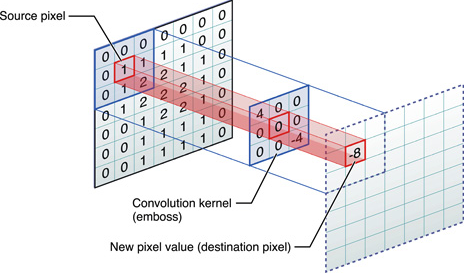
\includegraphics[width=0.5\textwidth]{gfx/kernel}
  \end{center}
  \caption{Convolutional kernel \cite{Apple}.
    The kernel gets centered on the source pixel and the convolution takes into account nearby pixels transforming the source pixel value.
    The convolution operation is a weighted sum of the source pixel with its nearby pixels. In this case:\\
    $(0\cdot4)+(0\cdot0)+(0\cdot0)
     +(0\cdot0)+(1\cdot0)+(1\cdot0)
     +(0\cdot0)+(1\cdot0)+(2\cdot-4) = -8$
  }
  \label{fig:sec:theory:covnets:kernel}
\end{figure}

\begin{figure}[t]
  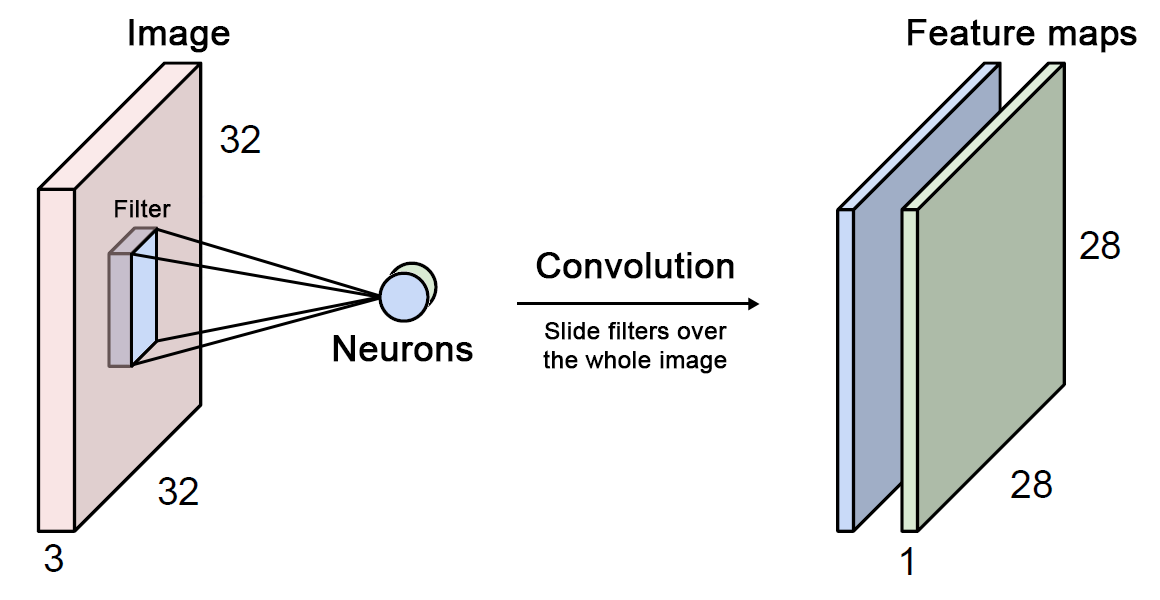
\includegraphics[width=\textwidth]{gfx/conv-layer-2}
  \caption{
    Anatomy of a convolutional layer and its output \cite{Guerzhoy2016}.
    On the left, the representation of an image of ${32}\times{32}$ pixels with $3$ color channels (\emph{RGB}).
    Neurons apply different filters of size ${5}\times{5}\times{3}$ in a particular region of the image.
    Together, all neurons applying the same filter within a layer produce what we call a feature map, resulting in as many as different filters are applied on the input.
    On the right, all produced feature maps combined become the input to the next layer as a ``new image'' of size ${28}\times{28}\times{N}$, being $N$ the number of filters in the layer.
  }
  \label{fig:sec:theory:conv-layer-2}
\end{figure}

\paragraph{Subsampling}
In the process of detecting higher-order features throughout subsequent layers of the network, the exact absolute position of detected features in feature maps is pretty much irrelevant compared to the relative position between them.
For instance, the pattern that describes the number $7$ is an endpoint in the upper left area of a horizontal segment, a corner in the upper right area, and an endpoint at the bottom of a vertical segment.
Still, small variations in the input may cause the pattern not to be detected because the features will not completely match the filter.
To make the network more robust against variations, the sensitivity of the convolutional layers has to be reduced.
This is effectively accomplished by reducing the resolution of the feature maps through non-linear \emph{subsampling} with pooling layers.
$Max$ is normally used as the non-linear function, giving the name of the subsampling operation \emph{max-pooling}, but it is not limited to it, as we will see in Chapter~\ref{chap:system}.
A pooling layer takes as input a volume of feature maps and, usually, has a non-overlapping filter of size ${2}\times{2}$ that gets applied on each one of the feature maps individually, as can be appreciated in Figure~\ref{fig:sec:theory:convnets:pooling}.
More specifically, the filter summarizes the feature map by performing max-pooling over its ${2}\times{2}$ regions and producing a single value for each, being this a size reduction of $75\%$.
It is important to note that this reduction applies only to the height and width of the original input since the depth refers to the number of feature maps and these are preserved.

\begin{figure}[t]
  \begin{subfigure}[b]{0.35\textwidth}
    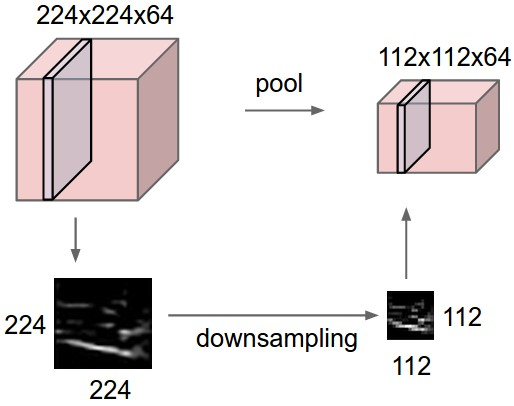
\includegraphics[width=\textwidth]{gfx/pool}
    \caption{General pooling}
    \label{fig:sec:theory:convnets:pooling:general}
  \end{subfigure}
  \hfill
  \begin{subfigure}[b]{0.55\textwidth}
    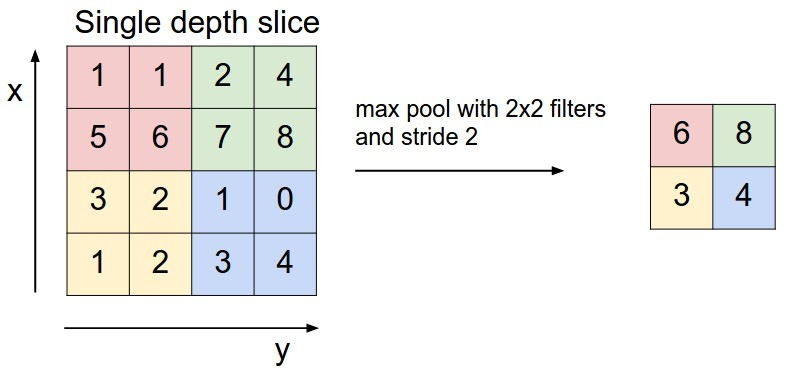
\includegraphics[width=\textwidth]{gfx/maxpool}
    \caption{Max-pooling}
    \label{fig:sec:theory:convnets:pooling:max}
  \end{subfigure}
  \caption{
    Overview of a pooling layer.
    On the left, the input and output of a pooling layer reducing only the height and width of the volume \cite{Karpathy}.
    On the right, a single feature map of the input volume being subsampled by non-overlapping ${2}\times{2}$ max-pooling \cite{Karpathya}.
  }
  \label{fig:sec:theory:convnets:pooling}
\end{figure}


\subsection{Architecture}
\label{sub:theory:convnets:achitecture}

While discussing the properties of CNNs, we introduced two of their building blocks: convolutional layers and pooling layers.
These alone are not enough to use CNNs for object recognition tasks since feature extraction is not the same as classification.
Let us have a look at how they fit in the big picture and the rest of the building blocks.

In Figure~\ref{fig:sec:theory:convnet} we present the typical configuration of a complete convolutional network.
We can see convolutional layers are alternated with pooling layers and ultimately fed into a fully-connected network.
Whereas convolutional layers generally increase the amount of feature maps making intermediate representations richer, pooling layers reduce their spatial resolution keeping the amount of parameters low and thus limiting overfitting.
After several convolutional-pooling layers, one final step is a fully-connected layer, where the classification finally takes place.
Optionally, normalization layers can be present after convolutional and pooling layers to increase the learning rate of the network.
During the learning process, the output of the classification at the end of the fully-connected layers is passed to a loss function that calculates the error of the prediction over a training sample.

\paragraph{Fully-connected layers}
The fully-connected layers is essentially a conventional fully-connected neural network only that we feed it with a set of feature maps produced by the convolutional layers, a highly-abstracted and rich representation of the original image at that point.
That means the data is much less noisy than raw pixels, so overfitting happens to a much lesser degree than what we discussed in \autoref{sec:theory:mlffnn:overfitting}.
Classification in the last layer is performed in the same fashion as we saw in \autoref{fig:sec:theory:mlffnn}, typically implemented as a $softmax$ layer that restricts the output to real values between 0 and 1, which summed add up to 1, representing the probability of the input belonging to the different classes.

\begin{figure}[t]
  \begin{center}
    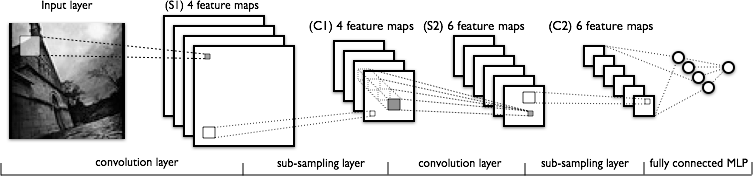
\includegraphics[width=\textwidth]{gfx/conv-network}
  \end{center}
  \caption{
    LeNet typical architecture \cite{Lisa2010}.
    On the left, there is an image (input layer).
    The image gets processed by a convolutional layer that extracts 4 elementary features producing 4 feature maps (S1).
    A pooling layer reduces the dimensionality while maintaining the same amount of feature maps (C1).
    Next, another convolutional layer extracts 6 higher-order features from the 4 feature maps (C2).
    Again, another pooling layer reduces the resolution of the 6 feature maps (S2).
    Finally, a fully-connected network takes the 6 feature maps and performs classification over them.
  }
  \label{fig:sec:theory:convnet}
\end{figure}

\paragraph{Normalization layers}
Additionally to these fundamental layers, normalization layers have been used as well, commonly referred to as \emph{Rectified Linear Units} or just \emph{ReLU}.
They simply use non-saturating activation functions like $max$ where the range is $[0,\infty]$, opposed to saturating activation functions like sigmoid where range $[0,1]$ to speed up the training phase \cite{Krizhevsky2012,Nair2010}.
The idea behind using non-saturating activation functions is minimizing the effects of the \emph{vanishing gradient problem} \cite{Socher2015}.
The vanishing gradient problem is a phenomenon in backpropagation that happens when weights adjust too slow on the first layers of very deep networks.
In them, the error contribution of each neuron in the initial layers will be very low and the saturating functions limit unnecessarily how much the weight can be adjusted.
Normalization layers, however, are falling out of use since it has been proved their contribution to the final result is very small and introduces new problems \cite{Lo2015}.

Summarizing, CNNs are mainly composed of convolutional layers, pooling layers, normalization layers and fully-connected layers.
Convolutional layers detect features in the input.
Pooling layers reduce the dimensionality of feature maps produced by convolutional layers.
Optionally, normalization layers magnify the non-linear properties of data to speed up learning.
Finally, fully-connected layers perform classification like we saw in \autoref{sec:theory:mlffnn}.


\subsection{Hyperparameters}
\label{sub:theory:convnets:achitecture}

In the next chapters, we will be looking at some already trained CNNs for image recognition.
Before we move on here is a quick recap of the architectural parameters that we will be talking about.

\paragraph{Convolutional input}
The shape of the receptive field in a convolutional layer.
It determines the local connectivity of neurons of the layer with neurons of the previous one.
It is normally larger in the first layer and it decreases for subsequent ones as the resolution decreases.
In image recognition tasks, it is common to range from $12x12$ to $15x15$ in the first layer.

\paragraph{Convolutional output}
The spatial arrangement of the output volume from a convolutional layer, which comes defined by \emph{depth}, \emph{stride}, and \emph{zero-padding}.
Depth represents how many neurons are connected to the same receptive field, each one applying a different filter.
It represents how many feature maps are produced as seen in \autoref{fig:sec:theory:convnets:conv-layer-1}.
Looking again at how convolution actually happens in \autoref{fig:sec:theory:covnets:kernel} will help to understand stride and zero-padding.
Stride defines how many units of separation the receptive field moves in the convolution operation and it represents the neuron density loss with respect to the previous layer.
With stride 1 there will be no ``gaps'' between neurons and their receptive field will be highly overlapped.
As stride goes up more ``gaps'' will appear, reducing the resolution of the output and making neurons' receptive field less overlapped.
Lastly, as seen in the convolution operation, the resolution of the result is smaller than the original on the edges.
Zero-padding is used to pad the output volume with zeros when maintaining the same resolution is required.

\paragraph{Pooling filter}
Shape of the filter in pooling layers, defined by height, width, and stride.
Usually $2x2$ filter with stride 2 are used, as in the example depicted in \autoref{fig:sec:theory:convnets:pooling:max}.
Stride is set to 2 so that the filters do not overlap.

% !TEX root = ../thesis.tex

\chapter{Context}
\label{chap:context}

\cleanchapterquote{No computer has ever been designed that is ever aware of what it's doing; but most of the time, we aren't either.}{Marvin Minsky}{(Father of the field of AI)}


% ------------------------------------------------------------------------------

In our journey to separation of form and content in neural networks, we will now go through the stepping stones that led to \citeauthor{Gatys2015B}'s Neural Style algorithm: 1) advances in object recognition using deep neural networks, 2) the development of techniques for visualizing intermediate processing steps within deep neural networks, and 3) the evolution of style transfer tasks.

In Chapter~\ref{chap:theory} we introduced convolutional neural networks (CNNs) and gave a glimpse of how they can be used for image recognition tasks.
In this chapter, we will describe, in detail, the challenges in object recognition and how CNNs, traditionally outperformed by other techniques, have become the state of the art.
Interestingly, it is not so well understood how some network architectures are better than others and, therefore, how current ones can be improved.
Also in this chapter, we will see a number of visualization techniques that have been recently developed with the intention of eliciting new intuitions to help us move forward in the field of neural networks, some of them with unexpectedly appealing results.
Considerations on their potential artistic implications quickly appeared, and so this chapter also covers an introduction to artistic rendering and a few influential style transfer techniques.


% ------------------------------------------------------------------------------

\section{Object Recognition}
\label{sec:context:object-recognition}

We refer to the task of general object recognition as recognizing any object in natural images and it has been a very difficult problem to solve until recently.
In \autoref{fig:sec:context:object-recognition} we can see a typical task of general object recognition on a natural image.
\citet{Pinto2008} concluded in 2008 that the difficulty of the task stems from the fact that any 3D object in the world has an infinite number of representations in 2D images, as position, pose, lighting, and background vary with respect to the observer.
At the same time, as we argued in Chapter~\ref{chap:intro}, the brain is able to perform general object recognition in the real world without any apparent struggle, and so replicating the human visual system started to be perceived as a possible strategy to fully capture the complexity of the task.

\begin{figure}[t]
  \begin{subfigure}[b]{0.5\textwidth}
    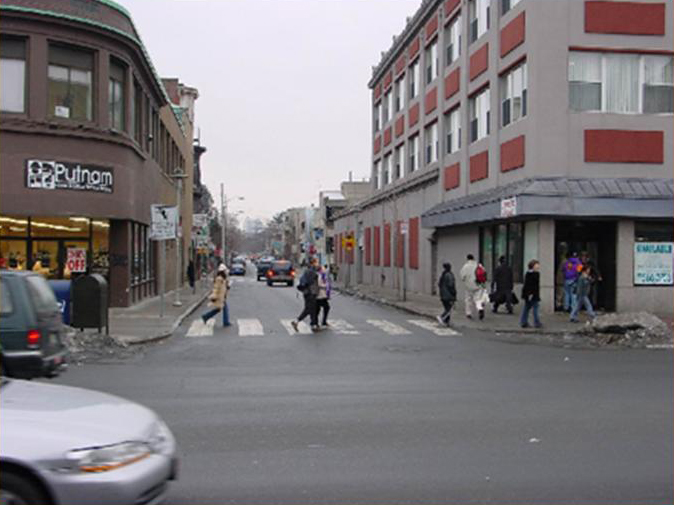
\includegraphics[width=\textwidth]{gfx/object-recognition-1}
    \label{fig:sec:context:object-recognition-1}
  \end{subfigure}
  \hfill
  \begin{subfigure}[b]{0.5\textwidth}
    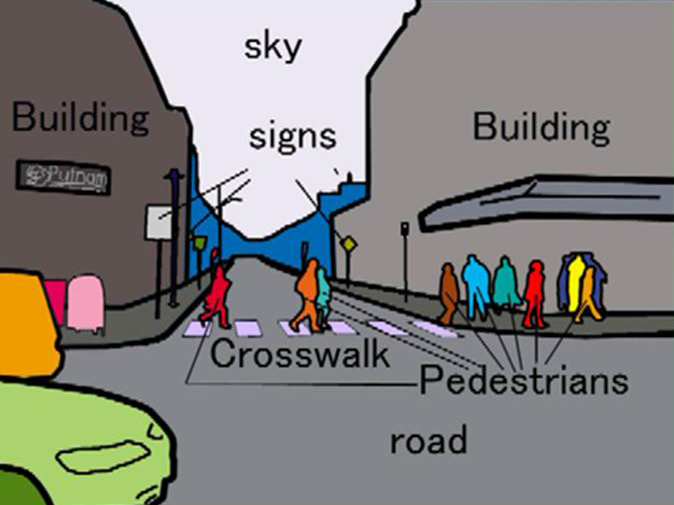
\includegraphics[width=\textwidth]{gfx/object-recognition-2}
    \label{fig:sec:context:object-recognition-2}
  \end{subfigure}
  \caption{
    Typical object recognition task \cite{Wolf}.
    Object recognition consists of locating objects on a natural image and giving them correct labels.
  }
  \label{fig:sec:context:object-recognition}
\end{figure}

As we mentioned in Chapter~\ref{chap:theory}, CNNs successfully emulate biological visual systems.
\citeauthor{LeCun2004B} in \cite{LeCun2004B} had already compared CNNs in 2004 with traditional techniques such as K-Nearest Neighbors and Support Vector Machines (SVM) for small-scale object recognition, finding that CNNs obtained better results in general and, especially, in non-normalized conditions.
\citeauthor{LeCun2004B} used the NORB dataset for training, being at that time the largest available one, with 97200 pre-processed image pairs of 50 different objects of 5 categories.

\citeauthor{Pinto2008} also argued NORB and other datasets available at that time, in the order of tens of thousands of images, such as Caltech-101/256 \cite{Fei-Fei2007,Griffin2007} or CIFAR-10/100 \cite{Krizhevsky2009}, were not large nor diverse enough to be used for general object recognition training.
They found systems trained with them were highly susceptible to the variations described above in this section (i.e. pose, position, lighting, etc.) and claimed that, for a learning system to be robust against them, it would need to capture the essence of the domain rather than rely on trivial regularities of the training samples.
Such a dataset, one that could consistently represent the domain (i.e. all the object in the real world without with all their variance), would not only required to be much larger than those available back in 2008 but also to contain unbiasedly-selected natural images.

Being clear the need for larger datasets at that point, ImageNet \cite{Deng2009} was handcrafted via crowdsourcing with the aim of organizing a fraction of the vast number of images on the Internet and making them available for object recognition tasks.
ImageNet is a large-scale, comprehensive, and diverse dataset of 15 million high-resolution accurately-labeled images, organized in a semantic hierarchy of 22000 categories.
In it, each noun in English, coming from the lexical database WordNet \cite{Wilkniss1998}, is associated with hundreds of clean images.
The achievements of ImageNet are two-fold.
On the one hand, the images depict representations of the words under many different perspectives and lighting conditions, allowing robustness against visual variability.
On the other hand, the hierarchical structure of the dataset makes it possible to interlink concepts, allowing algorithms to recognize several concepts at the same time (e.g. dog, therefore mammal and animal as well).

Based on the ImageNet dataset, the ImageNet Large-Scale Visual Recognition Challenge (ILSVRC) has established itself as the de-facto benchmark for object recognition algorithms.
Run as a yearly competition since 2010, it has triggered some of the most important advances in the field \cite{Russakovsky2015}.
Deep neural networks did not enter the scene until 2012.
CNNs had been terribly expensive to apply in large scale to high-resolution images until then, but \citet{Krizhevsky2012} finally managed to train a sufficiently large network for ILSVRC leveraging multiple GPUs.
They run a GPU-optimized implementation of 2D convolutional neural networks and used ImageNet as their training set, which was diverse enough to prevent severe overfitting.

The relevance of deep neural networks in object recognition tasks did nothing but increase in the last few years, as they keep getting the top scores each year at ILSVRC \cite{Russakovsky2015}.
At the time of writing this thesis, the use of GPU computing in deep neural networks is now generalized, facilitated by deep learning frameworks implementing GPU-optimized implementations of convolutions and all the necessary operations both for classification and training \cite{Bahrampour2015}.
Deep learning frameworks are just programming libraries that provide out-of-the-box tools for easily implementing deep neural networks, allowing researchers to focus on the architecture.
Some of the most popular ones currently are Caffe, developed by the Berkeley Vision and Learning Center \cite{Jia2014}; Theano, developed by l’Université de Montréal \cite{Bergstra2010}; TensorFlow, developed by Google \cite{Abadi2015}; or Torch, supported by Facebook and Nvidia \cite{Collobert2002}.

Deep learning frameworks have helped much to the reproducibility of experiments with neural networks, as they simplify the requirements for sharing architectures as well as trained models between researchers.
In Chapter~\ref{chap:system} we will see how the VGG network \cite{Simonyan2014}, one of the winners of ILSVRC 2014, rivaling human performance \cite{Russakovsky2015}, implemented in Caffe, and publicly available \cite{Simonyan2014web}, is used to effectively separate style and content.
Next, we will talk about the interest that grew for understanding what exactly happens within intermediate layers of CNNs trained for object recognition, resulting in a number of visualization techniques with surprising results.


% ------------------------------------------------------------------------------

\section{Visualization of Convolutional Neural Networks}
\label{sec:context:deep-visualization}

For a long time, neural networks have been perceived as ``black boxes''.
Although we can perceive the training phase as a simple function optimization process, trained models consist of a large number of trained non-linear parameters that we cannot easily comprehend in a sensible way \cite{Yosinski2015}.
Deep neural networks, like CNNs, are particularly difficult to study due to their size.
Learnable parameters in them are in the order of millions and this makes us understand very little about why some models work better than others.
Gaining insight into how trained models function is one way towards improving them, as new intuitions may arise or wrong assumptions may become apparent.

In an effort to shed some light, several studies have been done lately in the direction of providing techniques for visualizing different representations of what happens within CNNs trained for object recognition \cite{Dosovitskiy2015,Yosinski2015,Zeiler2014}.
We know each layer of trained CNNs extracts increasingly higher-level features of an input image until eventually, the last layer emits a decision of what was depicted in the image.
As we described in \autoref{sub:concepts:convnets:properties}, lower layers tend to extract edges or corners, while intermediate ones look for more complex elements like shapes, faces, or textures.
Finally, the last few layers use them to interpret high-level concepts like forests or streets.
Some of the visualization techniques we are about to see help us inspect how this actually happens.

\citet{Mahendran2014} study how to obtain different visualizations from the internal representations at intermediate CNN layers showing that, as expected, CNNs gradually build an increasing amount of tolerance towards variance.
This is visible in \autoref{fig:sec:context:deep-visualization:deep-visualization-reconstructions-1}, as representations of the initial monkey image become fuzzier, less specific layer after layer.
For constructing these visualizations, \citeauthor{Mahendran2014} use gradient descent to find a new image that matches the feature space at a particular layer in a very similar way as we will discuss in more detail in Chapter~\ref{chap:system}.
Interestingly, selecting different subsets of feature channels produces texturized versions of the original image, as shown in \autoref{fig:sec:context:deep-visualization:deep-visualization-reconstructions-2}.

\begin{figure}[b]
  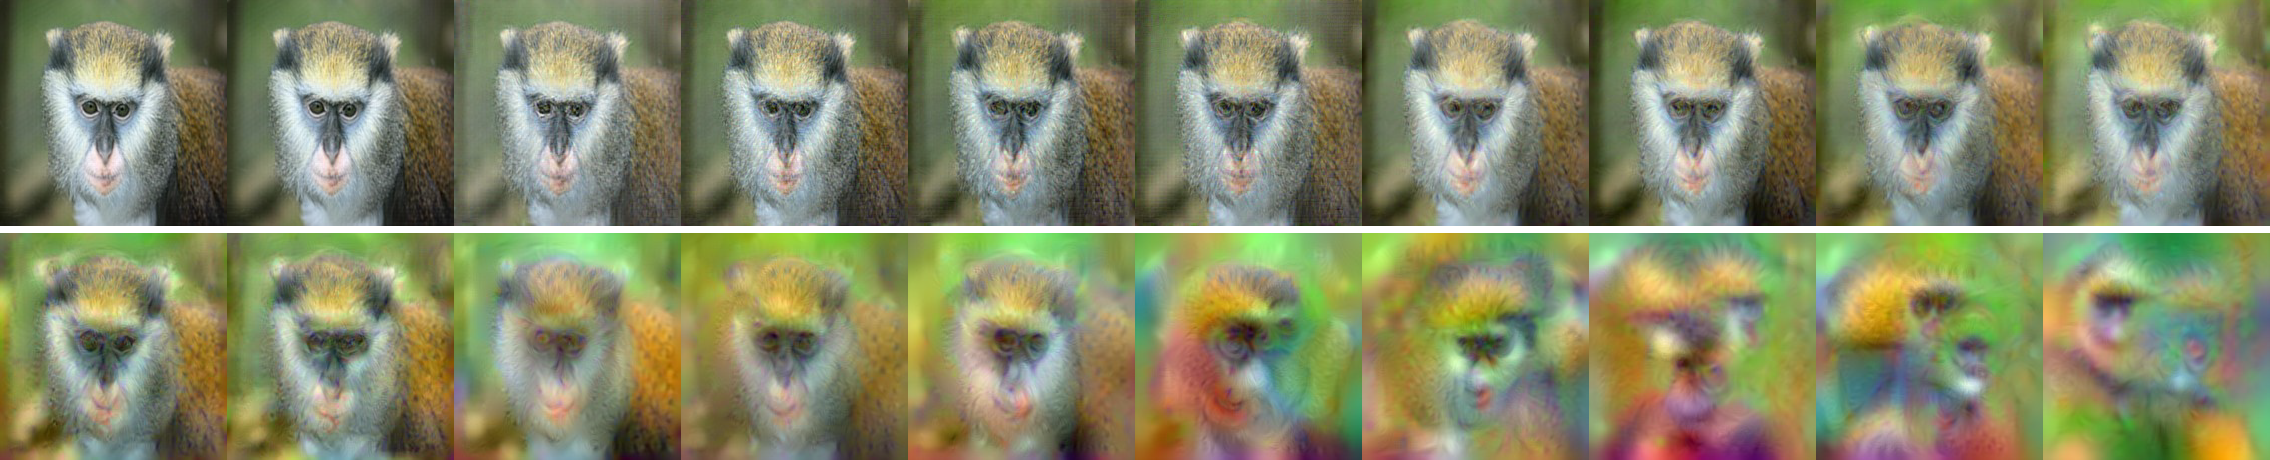
\includegraphics[width=\textwidth]{gfx/deep-visualization-reconstructions-1}
  \caption{
    CNN layer visualizations of a monkey image generated via gradient descent \cite{Mahendran2014}.
    Whereas the first layers (top row) maintain faithful representations of the original image, although increasingly fuzzy, invariance seems be appear in the last few ones (bottom row).
  }
  \label{fig:sec:context:deep-visualization:deep-visualization-reconstructions-1}
\end{figure}

\begin{figure}[t]
  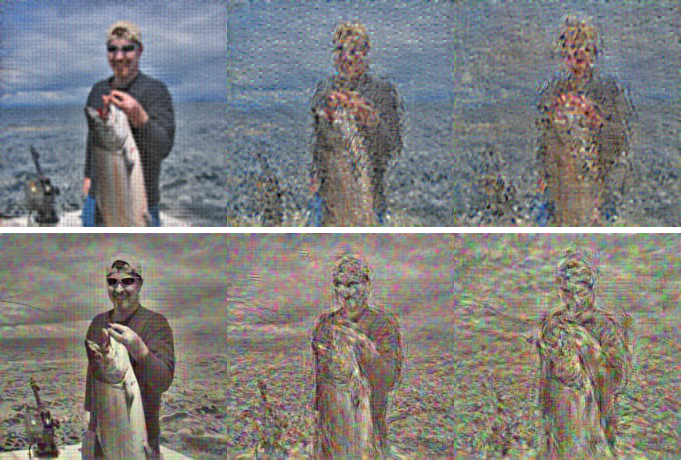
\includegraphics[width=\textwidth]{gfx/deep-visualization-reconstructions-2}
  \caption{
    CNN visualization of the first convolutional layer selecting different subsets of feature channels for the gradient descent generation \cite{Mahendran2014}.
    Depending on the selected channels, the visualizations are tuned towards different image parameters, producing texturized versions of the original image.
  }
  \label{fig:sec:context:deep-visualization:deep-visualization-reconstructions-2}
\end{figure}

\citet{Simonyan2014B} propose another visualization method, also through gradient descent, that generates class notions from a trained CNN.
That means a new image is generated in a way that the trained CNN would classify it with total certainty as the desired object.
In \autoref{fig:sec:context:deep-visualization-class}, some examples of this technique are displayed with clearly psychedelic results.
The generated images do not resemble natural images very much, more like graphic artifacts instead, but the network will anyway classify them correctly as these artifacts have been generated to cause precisely the right neural activations.

\begin{figure}[t]
  \begin{subfigure}[b]{0.3\textwidth}
    
\includegraphics[width=\textwidth]{gfx/deep-visualization-class-1}
    \caption{dumbbell}
    \label{fig:sec:context:deep-visualization-class-1}
  \end{subfigure}
  \hfill
  \begin{subfigure}[b]{0.3\textwidth}
    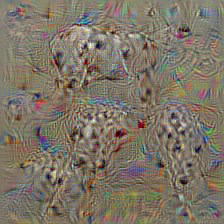
\includegraphics[width=\textwidth]{gfx/deep-visualization-class-2}
    \caption{dalmatian}
    \label{fig:sec:context:deep-visualization-class-2}
  \end{subfigure}
  \hfill
  \begin{subfigure}[b]{0.3\textwidth}
    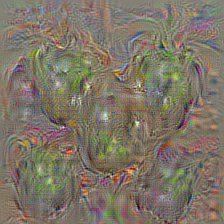
\includegraphics[width=\textwidth]{gfx/deep-visualization-class-3}
    \caption{bell pepper}
    \label{fig:sec:context:deep-visualization-class-3}
  \end{subfigure}
  \par\medskip
  \begin{subfigure}[b]{0.3\textwidth}
    
\includegraphics[width=\textwidth]{gfx/deep-visualization-class-4}
    \caption{keyboard}
    \label{fig:sec:context:deep-visualization-class-4}
  \end{subfigure}
  \hfill
  \begin{subfigure}[b]{0.3\textwidth}
    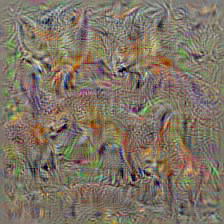
\includegraphics[width=\textwidth]{gfx/deep-visualization-class-5}
    \caption{kit fox}
    \label{fig:sec:context:deep-visualization-class-5}
  \end{subfigure}
  \hfill
  \begin{subfigure}[b]{0.3\textwidth}
    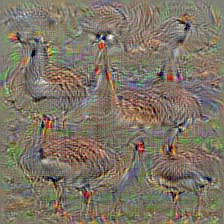
\includegraphics[width=\textwidth]{gfx/deep-visualization-class-6}
    \caption{goose}
    \label{fig:sec:context:deep-visualization-class-6}
  \end{subfigure}
  \caption{
    Images generated with gradient descent to artificially generate a desired classification, given a trained CNN \cite{Simonyan2014B}.
  }
  \label{fig:sec:context:deep-visualization-class}
\end{figure}

Google's DeepDream algorithm \cite{Mordvintsev2015} uses this same visualization technique to produce dream-like images in a process they call ``inceptionism'', useful for getting an idea of the level of abstraction a particular layer has achieved in its understanding of images.
DeepDream works as some sort of glorified \emph{pareidolia} that enhances whatever a trained CNN recognizes in an original image, replicating it in different sizes on every pass.
\autoref{fig:sec:context:deep-visualization:dream-buildings} shows images depicting scenery produced by DeepDream using random noise images as input and a CNN trained on places as the dreamer.
It can be explained because the a CNN trained on recognizing places has probably seen lots of structures, fountains and trees.
Also, because white noise images carry no information, we could say that these images are purely a product of the neural network's understanding of the world.

\begin{figure}[p]
  \begin{subfigure}[b]{\textwidth}
    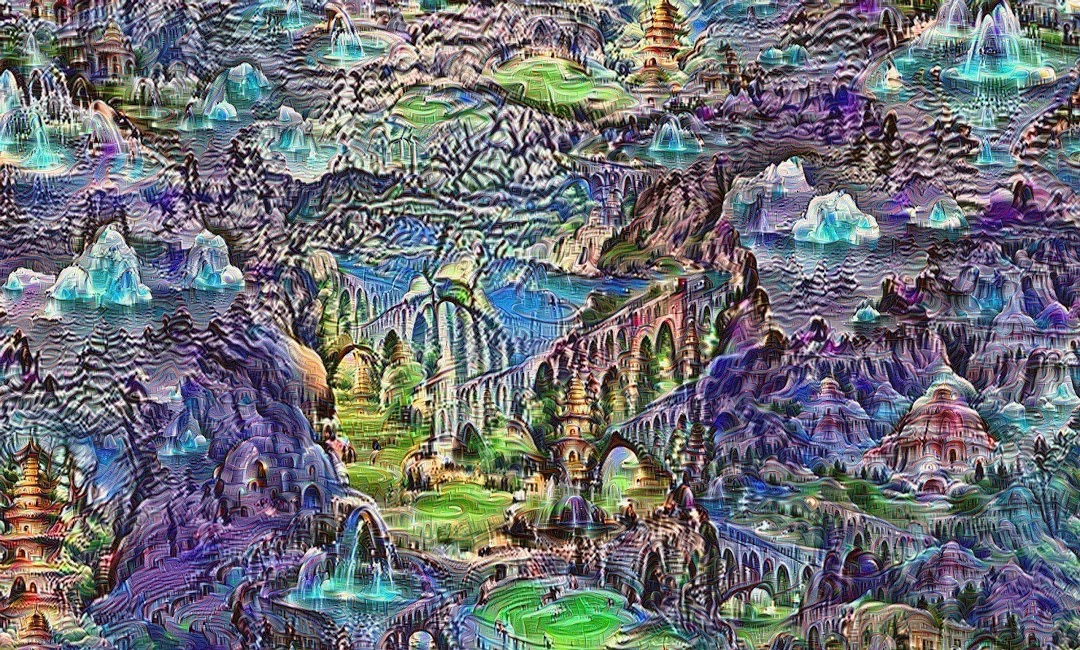
\includegraphics[width=\textwidth]{gfx/dream-buildings-1}
  \end{subfigure}
  \par\medskip
  \begin{subfigure}[b]{\textwidth}
    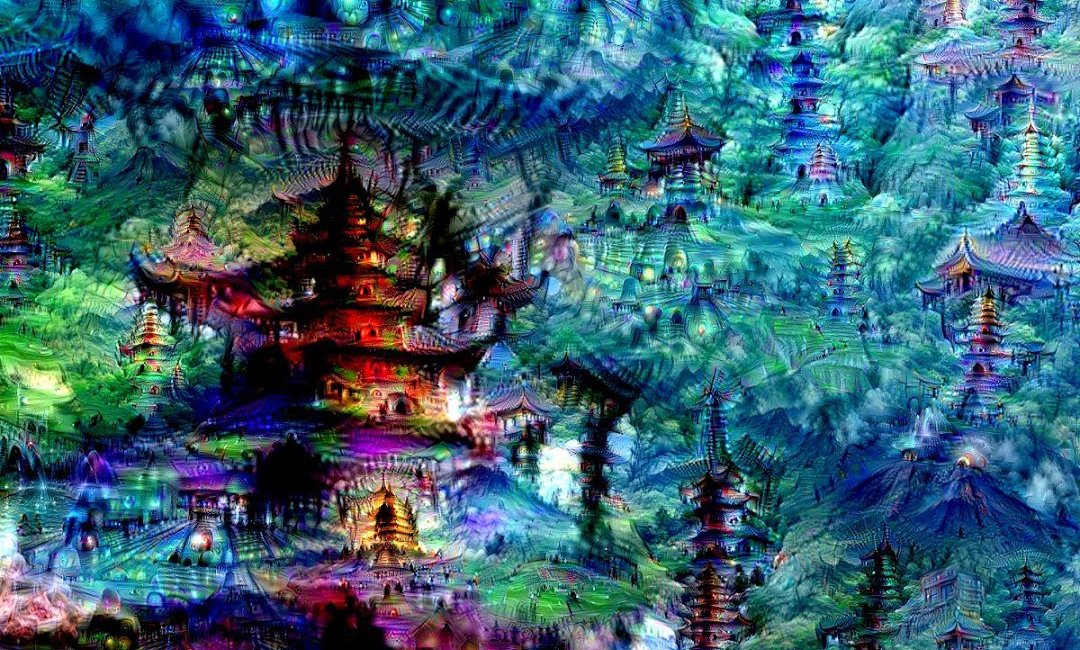
\includegraphics[width=\textwidth]{gfx/dream-buildings-2}
  \end{subfigure}
  \caption{
    Images generated with DeepDream from a white noise image and a CNN trained on places by the MIT Computer Science and AI Laboratory \cite{Mordvintsev2015}.
    Pagodas, fountains, bridges, and trees seem to be the most recurrent elements on them because the CNN was trained with thousand of images of them.
    Therefore, when ``dreaming,'' that is what the network sees.
  }
  \label{fig:sec:context:deep-visualization:dream-buildings}
\end{figure}

One final example of visualizations is given by \citet{Nguyen2014}, highlighting some of the problems of current CNN models.
Although they already rival human performance in many aspects, we can easily fool them by generated images that, by no means, resemble anything of what they claim to recognize.
For instance, in \autoref{fig:sec:context:deep-visualization:deep-visualization-fooling} we observe some of these fooling images that CNNs classify with total certainty as belonging to the categories shown below them.
These images have been generated with an evolutionary algorithm that applies random modifications and keeps those that better fit the desired category.

\begin{figure}[t]
  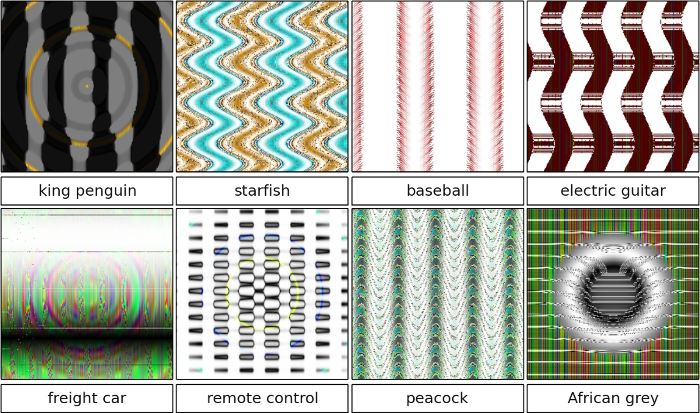
\includegraphics[width=\textwidth]{gfx/deep-visualization-fooling}
  \caption{
    Mislabeled images by a CNN trained for object recognition \cite{Nguyen2014}.
    Called ``fooling images'' and obtained with an evolutionary algorithm that applies random perturbations (mutation and/or crossover) on images and keeps those that produce the highest prediction in a desired category.
  }
  \label{fig:sec:context:deep-visualization:deep-visualization-fooling}
\end{figure}

All visualization methods described above hold some degree of artistic ``intention,'' as their respective authors observe.
First, \citeauthor{Mahendran2014}'s texturized images in \autoref{fig:sec:context:deep-visualization:deep-visualization-reconstructions-2} emerge naturally without the trained network having been encouraged to show it in any way.
Then, \citeauthor{Mordvintsev2015} speculate about the artistic implications of DeepDream, both as a rendering tool and as a step towards understanding the essence of the creative process in the human brain.
Lastly, \citeauthor{Nguyen2014} submitted some of these images to a selective art contest, the \emph{University of Wyoming 40th Annual Juried Student Exhibition}, got a third of them accepted, and some of them even received an award.

Artistic rendering, however, has been traditionally studied as a field of computer vision, and the problem of the separation of style and content was identified long ago as one of the main challenges for applying \emph{style transfer}.


% ------------------------------------------------------------------------------

\section{Style Transfer}
\label{sec:context:style-transfer}

We can understand artworks and paintings as the composition of form and content, as we commented in Chapter~\ref{chap:intro}.
Style transfer is the task of synthesizing a new stylized image with the same content as some source image and the style of a style sample.
To accomplish style transfer, not only the style-content combination is important, but even more so is the definition and extraction of style and content.
The difficulty of the latter is intrinsic to the separation of style and content, which is a very fundamental problem, since not even in the history of art literature seems to be a consensus as to what is content and what is style \cite{Xie2007}.

Because of this fundamental difficulty, we cannot use any formally-described evaluation for style transfer, and so we resort to appealing the human visual system as it will be the ultimate consumer of the generated images \cite{Lin2011}.
The main criteria commonly used are the score from an \emph{artistic Turing test} and the \emph{perceptual quality}.
Whereas the artistic Turing test score will be higher the more difficult it is for humans to distinguish generated images from those created by hand \cite{Kyprianidis2013}, the perceptual quality refers to the subjective degree of similarity with the original images providing content and style.

Style transfer is studied in the field of \emph{non-photorealistic rendering}, in development since the late 1980s as a branch of computer vision, which attempts to provide tools for mimicking the style of paintings or animated cartoons in digital art, both in 2D and 3D \cite{Lee2010, Kyprianidis2013}.
Non-photorealistic rendering has become a highly multidisciplinary field, being influenced by progress done in computer graphics, perceptual modeling, and human-computer interaction.
We will focus only on small collection of 2D image-based style transfer techniques.
In particular, we will analyze those based on texture synthesis most closely related to Neural Style \cite{Gatys2015B}.

Style transfer is often approached as a texture transfer operation, sharing many of the challenges of texture synthesis \cite{Ashikhmin2003}.
Given a small texture example, texture synthesis algorithms try to generate a texture of arbitrary size.
On the other hand, texture transfer takes a target image and a texture source and modifies part of the target image with information with the given texture, while trying to maximize the perceptual quality of the result.

\citet{Hertzmann2001} proposed in 2001 a statistical-based method for style transfer called Image Analogies.
It generates a new image $B'$ that relates to $B$ in the same way as $A'$ relates to $A$, being $A$, $A'$, and $B$ the inputs to the system and $B'$ the output.
Conceptually, given an image $A$ and its filtered version $A'$, the system learns the transformation $A \mapsto A'$ and applies it to a target image $B$ to create an analogously filtered image $B'$.
\autoref{fig:sec:context:style-transfer:style-transfer-analogy} shows the algorithm at a glance.
The limitation of this approach is clear, as both an original image and its artistic version are required.

\begin{figure}[t]
  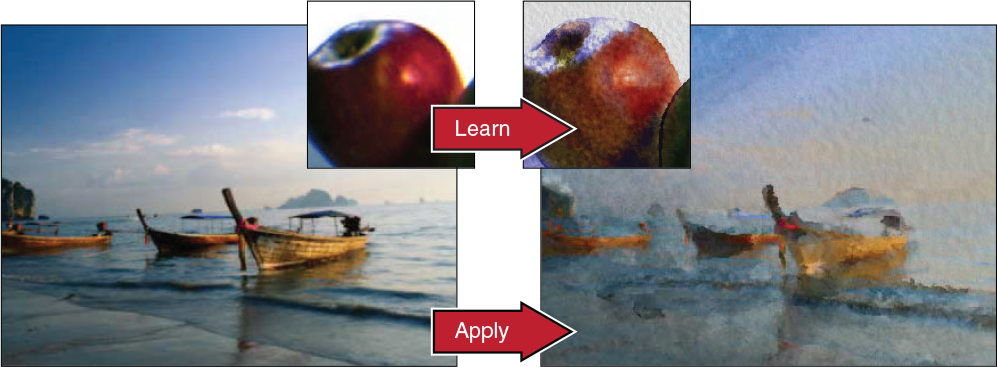
\includegraphics[width=\textwidth]{gfx/style-transfer-analogy}
  \caption{
    The Image Analogies algorithm \cite{Hertzmann2001}.
    Given the apple image and its filtered version, the algorithm learns the luminance transformation that must be applied to the boats image to produce an analogous filtered new image.
  }
  \label{fig:sec:context:style-transfer:style-transfer-analogy}
\end{figure}

Later, in 2003, \citet{Ashikhmin2003} developed an algorithm called Fast Texture Transfer that produces similar results but requires only a single texture sample.
The algorithm uses \emph{Markov random fields} to model the sample texture and then it generates the stylized image by growing texture patches, blending them pixel by pixel with those of the target image.
A limitation of this style transfer approach, also shared with \citeauthor{Hertzmann2001}'s, is that texture coherence can only be preserved locally \cite{Lee2010} and, thus, only small texture patches are applied, as shown in \autoref{fig:sec:context:style-transfer:style-transfer-analogy}.

\begin{figure}[t]
  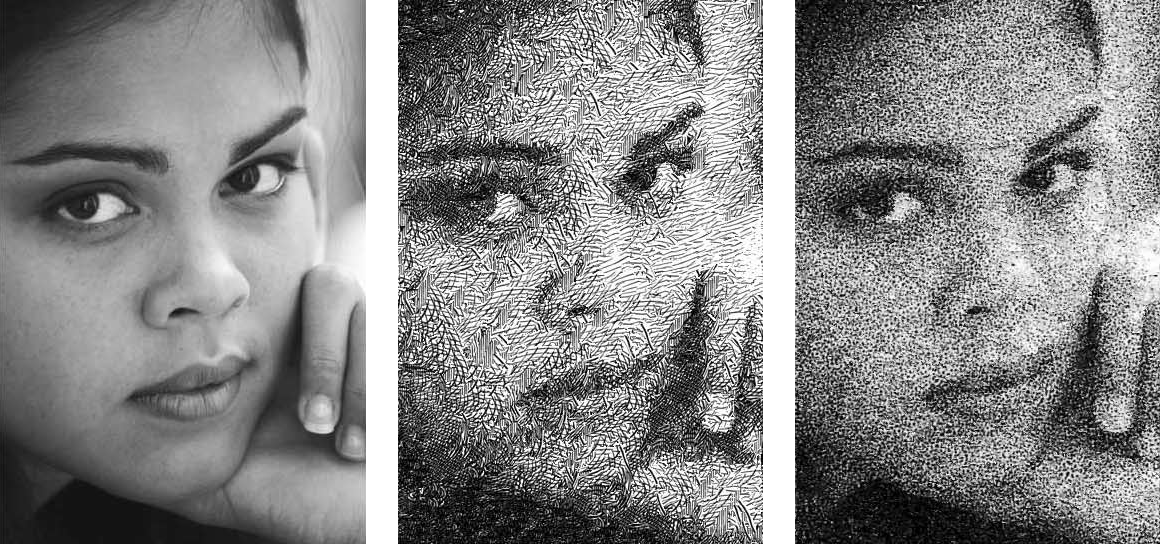
\includegraphics[width=\textwidth]{gfx/style-transfer-fast-texture}
  \caption{
    Results of applying Fast Texture Transfer with different texture samples \cite{Ashikhmin2003}.
    At the left, the target image on which the style is applied.
    At the center, the target image with a hatching drawing texture applied.
    At the right, the target image with a charcoal drawing texture applied.
  }
  \label{fig:sec:context:style-transfer:style-transfer-analogy}
\end{figure}

\citet{Xie2007} proposed in 2007 a new method called Feature Guided Texture Synthesis (FGTS) that better preserves the content of the target image, as we can observe in \autoref{fig:sec:context:style-transfer:style-transfer-feature}.
In this algorithm, first, a feature field is calculated from the target image trying to find edges and corners, assuming those pixels carry more information for the human visual system.
Then, a style transfer process similar to the previous one applies the texture but preserves the pixels specified in the feature field.
This method, like the ones described before, uses low-level statistical features.
\citeauthor{Xie2007} already mentioned the disadvantage of this and anticipated a sharper separation of style and content using higher-level, larger-scale features involving prior human knowledge.

\begin{figure}[t]
  \begin{subfigure}[b]{0.24\textwidth}
    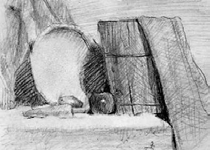
\includegraphics[width=\textwidth]{gfx/style-transfer-feature-1}
    \caption{Style example}
  \end{subfigure}
  \begin{subfigure}[b]{0.24\textwidth}
    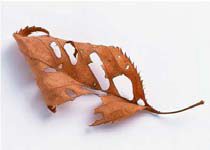
\includegraphics[width=\textwidth]{gfx/style-transfer-feature-2}
    \caption{Target image}
  \end{subfigure}
  \hfill
  \begin{subfigure}[b]{0.24\textwidth}
    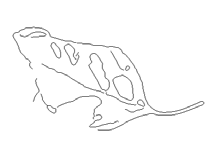
\includegraphics[width=\textwidth]{gfx/style-transfer-feature-3}
    \caption{Feature image}
  \end{subfigure}
  \begin{subfigure}[b]{0.24\textwidth}
    
\includegraphics[width=\textwidth]{gfx/style-transfer-feature-4}
    \caption{Feature field}
  \end{subfigure}
  \par\medskip
  \begin{subfigure}[b]{0.5\textwidth}
    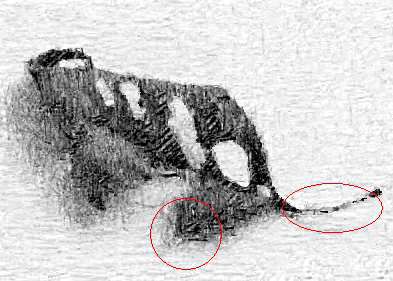
\includegraphics[width=\textwidth]{gfx/style-transfer-feature-5}
    \caption{Analogies}
  \end{subfigure}
  \begin{subfigure}[b]{0.5\textwidth}
    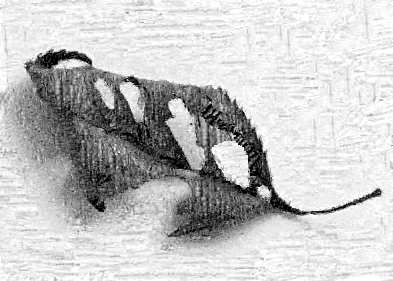
\includegraphics[width=\textwidth]{gfx/style-transfer-feature-6}
    \caption{FGTS}
  \end{subfigure}
  \caption{
    Comparison between Image Analogies and Feature Guided Texture Synthesis \cite{Xie2007}.
    On the top row, from left to right: the style example (a) to be transferred to the target image (b), the computed features from the target image (c), and the feature field defining which pixels carry the most content information and therefore should be preserved (d).
    Bottom left (e), the result produced by image analogy with the most severe content losses highlighted in red.
    Bottom right (f), the result produced by FGTS without the content losses seen in (e).
  }
  \label{fig:sec:context:style-transfer:style-transfer-feature}
\end{figure}

Lastly, in 2010, \citet{Lee2010} proposed an improved method called Directional Texture Transfer that finally transferred larger-scale patterns.
The algorithm attains this goal by taking into account the flow of a target image and interpolating it with that of a style source, using the result as the guide to place brush strokes.
We can see in \autoref{fig:sec:context:style-transfer:style-transfer-directional} how this approach preserves the different regions of the target image very sharply, as the strokes are transferred with different intensity.
This method creates compelling results, but it is limited to stroke-based rendering and far from the generalization we are looking for in a holistic separation of style and content.

\begin{figure}[t]
  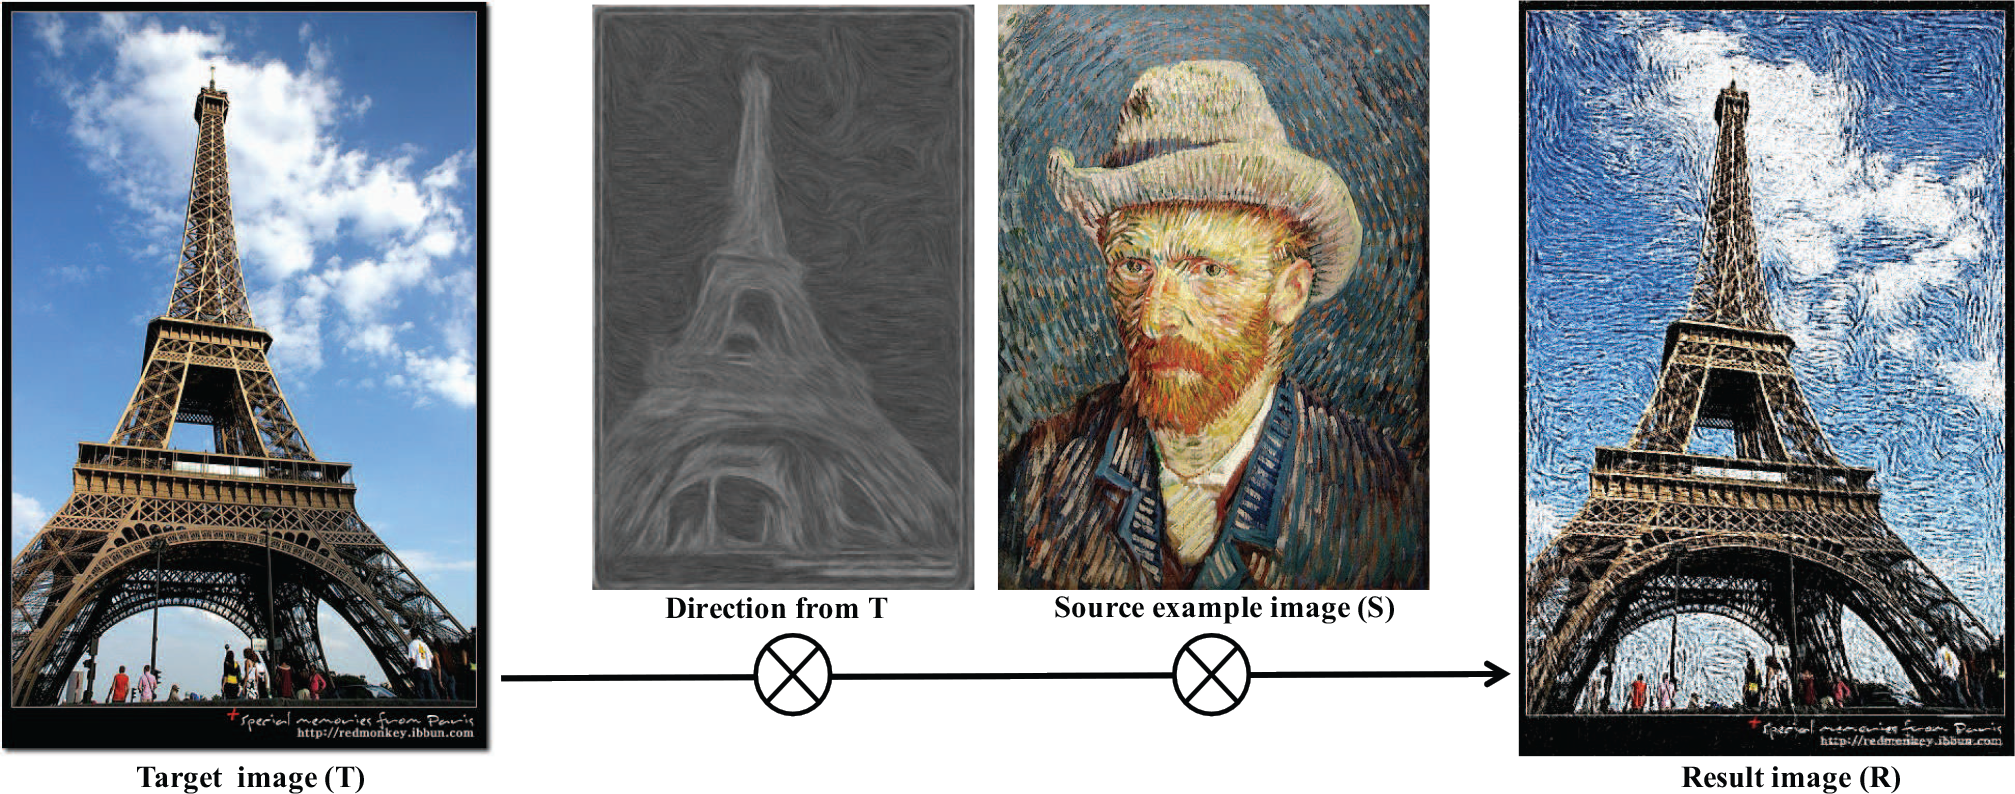
\includegraphics[width=\textwidth]{gfx/style-transfer-directional}
  \caption{
    Results of applying Directional Texture Transfer \cite{Lee2010}.
    First, the flow of the target image (T) is calculated and then interpolated with that of the style source (S), eventually used to guide the strokes that compose the result image (R).
  }
  \label{fig:sec:context:style-transfer:style-transfer-directional}
\end{figure}

\citeauthor{Kyprianidis2013}, in a style transfer techniques survey \cite{Kyprianidis2013} published in 2013, identified a clear tendency towards global-scope approaches, like \citeauthor{Lee2010}'s, rather than to local-level statistical measurements, like the first three ones we discussed in this section.
Global scope approaches require taking larger-scale patterns into account, which is, precisely, what deep neural networks trained for object recognition are very good at.
Two years after \citeauthor{Kyprianidis2013}'s survey, \citeauthor{Gatys2015B}'s Neural Style algorithm \cite{Gatys2015B}, resorted to deep neural networks and outperformed every other technique used in style transfer to date.
Even more interesting, it has given us a way to crack open the problem of separation of style and content.

% !TEX root = ../thesis.tex

\chapter{Neural Style}
\label{chap:system}

\cleanchapterquote{Sometimes a problem that initially looks hopelessly complicated turns out to have a surprisingly simple solution.}{Nick Bostrom}{(Superintelligence: Paths, Dangers, Strategies)}

\todo[inline]{Connect with previous chapter}

% Separation of content and style, as we discussed in the introduction, has not been traditionally a matter of concern for pattern recognition in machine learning.
% Although object recognition
% As we have seen also in chapter 3, attempts at style transfer rely on pixel-wise operations.

% Neural Style is not the first attempt at extracting style from artworks
% Features from Deep Neural Networks trained on object recognition have been previously used for style recognition in order to classify artworks according to the period in which they were created.20 There, classifiers are trained on top of the raw network activations, which we call content representations. We conjecture that a transformation into a stationary feature space such as our style representation might achieve even better performance in style classification.
% \cite{Karayev2014}

% As discussed in Chapter~\ref{chap:intro}, style has received little attention in pattern recognition.

\citeauthor{Gatys2015B} proved in \cite{Gatys2015B} content and style in convolutional neural networks are separable.
They proposed an algorithm that not only is able to do so but can manipulate both representations independently to produce new perceptually meaningful images.
Some examples of the results achieved by their algorithm can be seen in \autoref{sub:system:examples}.

\begin{figure}[!htb]
  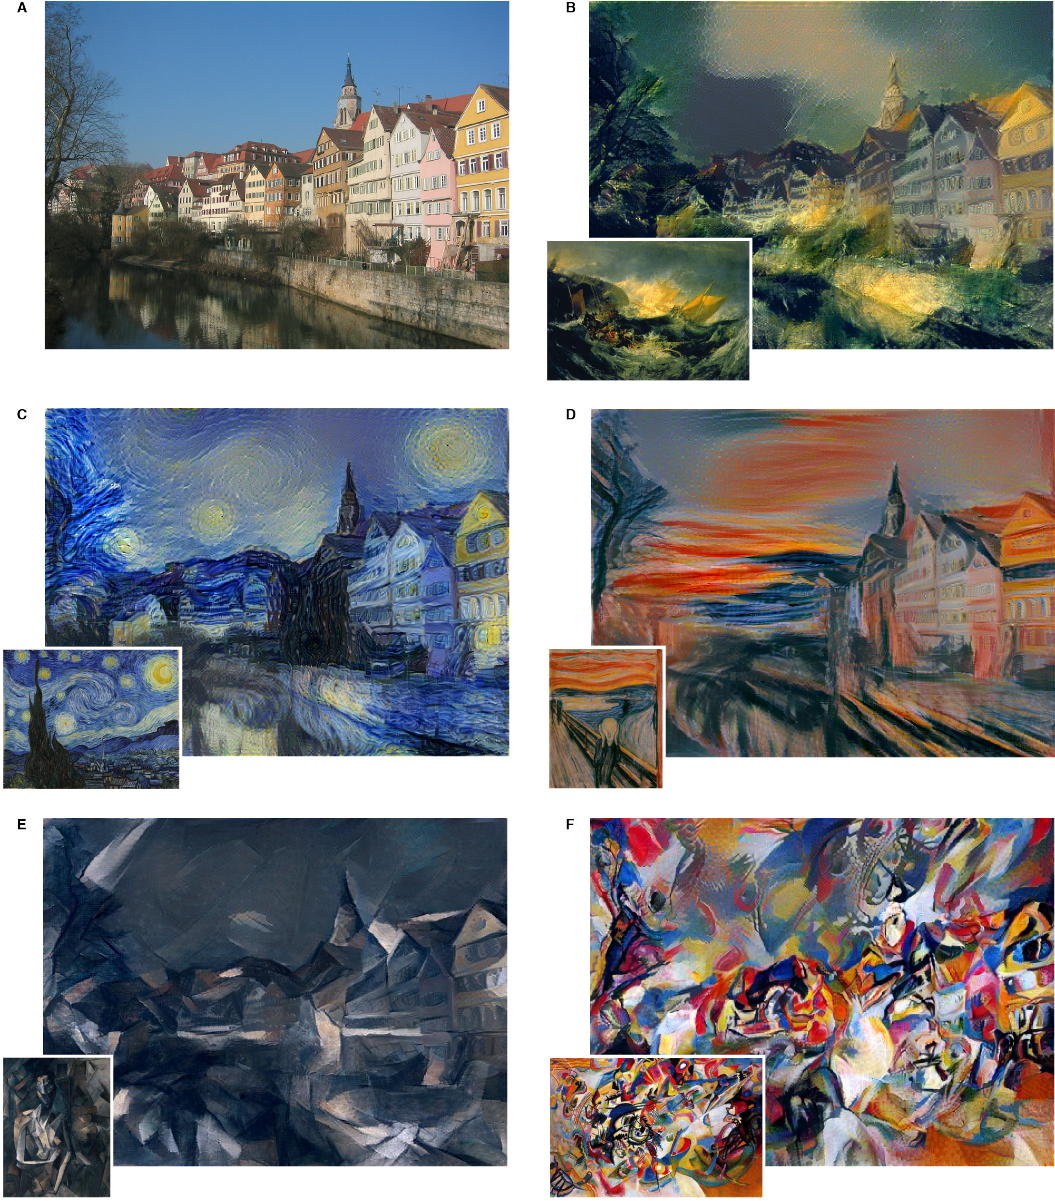
\includegraphics[width=\textwidth]{gfx/neural-style-examples}
  \caption{
    Images synthesized using the neural style algorithm \cite{Gatys2015B}.
    In \textbf{A}, the original photograph, depicting the Neckarfront in T\"ubingen, Germany, (shot by Andreas Praefcke).
    The style is applied from different artworks, shown in the bottom left corner of each panel.
    \textbf{B} \emph{The Shipwreck of the Minotaur} by J.M.W. Turner, 1805.
    \textbf{C} \emph{The Starry Night} by Vincent van Gogh, 1889.
    \textbf{D} \emph{Der Schrei} by Edvard Munch, 1893.
    \textbf{E} \emph{Femme nue assise} by Pablo Picasso, 1910.
    \textbf{F} \emph{Composition VII} by Wassily Kandinsky, 1913.
  }
  \label{sub:system:examples}
\end{figure}

In these examples we observe the style from several artworks is transferred to an original photograph.
The content of the photograph, its global arrangement, is effectively preserved while the style of the artworks, color, patterns, and local structures, is blended.
Unlike other attempts in style transfer, \todo{Check later}{as we have seen before}, neural style uses the feature space from a convolutional neural network trained in object recognition.


% ------------------------------------------------------------------------------

\section{Method}
\label{sec:system:method}

Neural style, simply put, takes two image sources: a photograph and an artwork, extracts the content from one and the style from the other, and generates a new image that matches both simultaneously.
The whole algorithm relies on a CNN already trained in object recognition to extract content and style from features found in source images.

\todo[inline]{Consider moving/connecting VGG-Network details to previous chapter}

\citeauthor{Gatys2015B}'s particular implementation uses VGG-Network \cite{Simonyan2014}, a CNN already trained in object recognition.
VGG-Network was designed and trained by the Visual Geometry Group at the University of Oxford with the goal of evaluating the performance of networks with increasing depth and it managed to score top results in ImageNet Challenge 2014.
The network achieved best results in between 16 and 19 weight layers with an architecture of convolutional filters with a very small receptive field (${3}\times{3}$, the smallest that can capture the notion of left/right, up/down and center) stride set to 1 pixel, and zero-padding to 1 pixel as well to preserve the original resolution of the input after the convolution.
Subsampling is performed by 5 max-pooling layers, inserted after some of the convolutional layers, over a ${2}\times{2}$ pixel window with stride set to 2 pixels so that the filter does not have overlapping input.

The VGG-Network implementation in Caffe framework is available under Creative Commons Attribution License \cite{Simonyan2014web}.
Among the 19-layer VGG-Network, neural style uses all 16 convolutional and 5 pooling layers, but none of the fully-connected layers, since classification is not required.
Max-pooling is replaced by average pooling because it produces a smoother gradient flow \cite{Boureau2010} and it results in cleaner synthesized images.
Lastly, for practical reasons, the weights in the networks are rescaled such that the mean activation of each filter over images and positions is equal to one.
Rescaling weights in this manner is always possible without affecting the output of the CNN when the activation functions are normalized with a ReLU layer like is the case in VGG-Network.

In a bit more detail, these are the algorithm's main stages: 1) both images get processed by the VGG-Network to produce their feature spaces, 2) content and style are extracted from those, and finally 3) a new image that matches them both is generated through backpropagation.

We will focus next on what we mean by content and style exactly and then how VGG-Network can synthesize new images that match content or style representations from a source image.
At the end, it will be obvious how it is possible to transfer the style using the neural style algorithm.


\subsection{Feature Representations}
\label{sub:system:method:representations}

Content and style of an image in neural style is characterized making use of the feature space produced by the VGG-Network.
If we remember the introduction on CNNs discussed in \autoref{sec:theory:convnets}, an original input gets transformed by filters defined in each layer as it moves across the network during the feed-forward phase.
To be more precise, a layer produces as many feature maps as filters it defines, each one of them highlighting different features of the input and represented by neural activations.
Spatially, we can imagine the output from a layer as a volume in which each slice is a feature map where neuron responses are arranged in 2D grids.
In image recognition tasks, each feature map is actually another image where pixels are active wherever the feature captured by the associated filter is present.

\paragraph{Content Representation}
We can also understand it the other way around, perceiving neural activations at a certain layer as an abstract representation of the original input image.
As a result of the VGG-Network having been trained in object recognition, its learned filters capture spatial information of the original input image, and thus, we can talk of the neural activations from a CNN layer as the content representation.
Formalizing it for an input image $\vec{x}$, let $l$ be a layer that applies $N_l$ different filters and produces $N_l$ feature maps of size $M_l$, where size is defined by the resolution ${height}\times{width}$ of the feature maps.
Vectorizing the feature maps, the total neural response at layer $l$ can be stored in a 2D matrix $F^l \in \mathbb{R}^{{N_l}\times{M_l}}$ where $F^l_{ij}$ is the feature activation for the $i^{th}$ filter at neuron $j$.

\begin{equation}
  F^l =
  \underbrace{
    \begin{bmatrix}
      F^l_{11}   & F^l_{12}   & \dots  & F^l_{1M_l} \\
      F^l_{21}   & F^l_{22}   & \dots  & F^l_{2M_l} \\
      \vdots     & \vdots     & \ddots & \vdots   \\
      F^l_{N_l1} & F^l_{N_l2} & \dots  & F^l_{N_lM_l}
    \end{bmatrix}
  }_{\text{vectorized feature maps}}
  \begin{matrix*}[l]
    \leftarrow & \text{filter } 1 \\
    \leftarrow & \text{filter } 2 \\
    \vdots                     \\
    \leftarrow & \text{filter } N_l
  \end{matrix*}
\end{equation}

\paragraph{Style Representation}
VGG-Network, as stated before, was not trained in any kind of style recognition task, so it is clear there is no style representation of any sort directly available in the network.
Nonetheless, \citeauthor{Gatys2015A} described in a previous work \cite{Gatys2015A} a method to build a style representation on top of the content representations without having to modify the network.
While the concept of content representation is somewhat intuitive to comprehend, style representation will require us to take a short detour to explain what we mean with style and what we expect its representation to be.

\citeauthor{Gatys2015A} approach style as a texture.
Texture synthesis tries to extract a texture model from an initial example so that arbitrary new samples of textures can be produced from it.
The quality of the model is normally evaluated by how hard it is for human inspection to distinguish between original and generated.
A texture model cannot be described by its exact pixel representation, rather a texture model must be uniquely described by statistical measurements, referred to as summary statistics, as was originally proposed by \citet{Julesz1962}.
We can understand this better by looking at \autoref{sub:system:method:style-reconstruction:texture}, showing a randomly generated image with 4 levels of brightness where a different texture has been applied on either half.
On the one hand, it illustrates how textures are independent of exact pixel representation as the randomly generated grid does not affect our ability to distinguish both textures.
On the other hand, it proves summary statistics are a better metric to distinguish one pattern from another.
This means that, within a texture model, any image that presents the same summary statistics as another, although having a different exact representation, can be considered the same texture.

\begin{figure}[htb]
  \begin{subfigure}[b]{0.5\textwidth}
    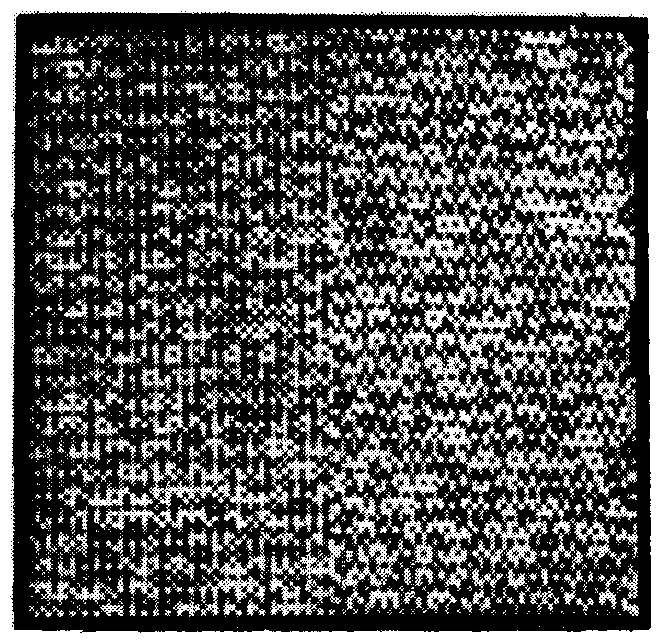
\includegraphics[width=\textwidth]{gfx/texture-1}
    \caption{Two-texture image}
    \label{sub:system:method:style-reconstruction:texture-1}
  \end{subfigure}
  \hfill
  \begin{subfigure}[b]{0.5\textwidth}
    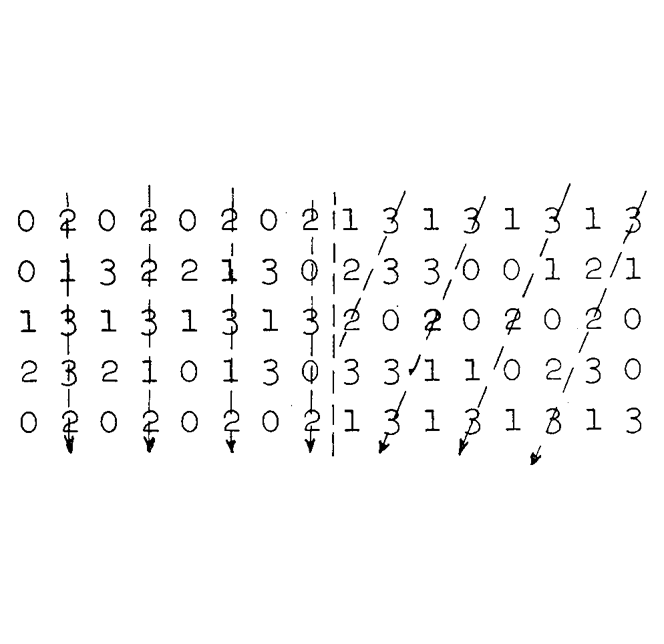
\includegraphics[width=\textwidth]{gfx/texture-2}
    \caption{Texture pattern generation}
    \label{sub:system:method:style-reconstruction:texture-2}
  \end{subfigure}
  \caption{Pattern discrimination \cite{Julesz1962}.
    On the left (a), an image with two different textures clearly visible.
    On the right (b), the pattern used to generate different textures on both halves of the image.
    Numbers represent the level of brightness and those outside of the arrows are randomly distributed.
    While no two regions on either half of the image are the same (brightness random distribution), the underlying patterns existing on each half (arrows) make them clearly distinguishable.}
  \label{sub:system:method:style-reconstruction:texture}
\end{figure}

Texture synthesis was later inspired by human visual systems, using Gabor filters for edge detection, which proved to be very similar to the human visual system \cite{Heeger1995,Portilla2000} and statistical measurements in these cases were taken over Gabor filter responses rather than on image pixels.
Results presented by \citet{Portilla2000} are probably still the best produced to date \cite{Gatys2015A}, but the method required careful handcrafting summary statistics that would result in good texture models.
Because of this, \citeauthor{Gatys2015A} argued \citeauthor{Portilla2000}'s method fails to generalize the full extent of natural textures and proposed in \cite{Gatys2015A} a method that combines the use of summary statistics with the feature space of a CNN already trained in object recognition, which fully models the human visual system.

Picking up again the analogy between textures and style, the summary statistic of the texture model is what we refer to as the style representation.
Since textures models are per definition stationary, the style representation must discard the spatial information existing in feature maps while keeping the notion of patterns.
One way to achieve it is by calculating the correlations between features maps in a CNN layer.
We can, therefore, formalize the style representation of an image $\vec{x}$ as a set of per-layer feature correlations $\{G^1, G^2, \dots, G^L\}$, where per-layer feature correlations are stored in 2D Gram matrixes $G^l \in \mathbb{R}^{{N_l}\times{N_l}}$ \cite[Theorem~7.2.10]{Horn2012}:

\begin{equation}
  G^l =
  \begin{bmatrix}
    G^l_{11}   & G^l_{12}   & \dots  & G^l_{1N_l} \\
    G^l_{21}   & G^l_{22}   & \dots  & G^l_{2N_l} \\
    \vdots     & \vdots     & \ddots & \vdots   \\
    G^l_{N_l1} & G^l_{N_l2} & \dots  & G^l_{N_lN_l}
  \end{bmatrix}
\end{equation}

Being $G^l_{ij}$ the inner product between the vectorized feature maps $i$ and $j$ in layer $l$, representing their degree of correlation:

\begin{equation}
  G^l_{ij} =
  \begin{bmatrix}
    F^l_{i1} & \dots & F^l_{iM_l}
  \end{bmatrix}
  \begin{bmatrix}
    F^l_{j1} \\
    \vdots \\
    F^l_{jM_l}
  \end{bmatrix}
  = \sum_k F^l_{ik}F^l_{jk}
\end{equation}

Having defined content and style representations we can now move to discussing how they can be used to produce new images.
\citeauthor{Gatys2015B} refer to this process feature reconstruction.


\subsection{Feature Reconstruction}
\label{sub:system:method:reconstructions}

In neural style algorithm, feature reconstruction is the process of visualizing some feature representation of an original input image.
The visualization is, in fact, a new image $\vec{x}$ that must be generates so that either its content representation or its style representation matches that of the original input image.
We will talk about \emph{content reconstruction} when the new image $\vec{x}$ is generated so that matches the content representation and \emph{style reconstruction} when it does so with the style representation.
The strategy to generates the new image $\vec{x}$ is approaching the task as an optimization problem very much like backpropagation, as we will see next.

\paragraph{Content reconstruction}
Starting from a random white noise image $\vec{x}$, we want to transform it so that it becomes the image $\vec{x}$ whose content representation is the same as the original photograph $\vec{p}$ at a certain layer $l$.
It is then the difference between content representations of $\vec{x}$ and $\vec{p}$ what we need to minimize.
So, let $P^l$ and $F^l$ be the content representations of the original photograph $\vec{p}$ and the generated image $\vec{x}$, respectively, in layer $l$, we define the loss function to be minimized as the squared error between the two representations:

\begin{equation}
  \mathcal{L}_{content}(\vec{p}, \vec{x}, l) = \frac{1}{2} \sum_{i,j}(F^l_{ij}-P^l_{ij})^2
\end{equation}

With this loss function we want to ultimately modify the white noise image $\vec{x}$, which can be perceived as the content representation at the input layer $l = 0$, so we can say we want to find the partial derivative of the loss with respect to the content representation such as:

\begin{equation}
  \Delta \vec{x} =
  \frac{\partial \mathcal{L}_{c}}{\partial \vec{x}} =
  \frac{\partial \mathcal{L}_{c}}{\partial F^0}
\end{equation}

Which generalized for any layer $l$ with the chain rule can be analytically calculated for every neuron as:

\begin{equation}
  \mathcal{L}^l_{ij} =
  \frac{\partial \mathcal{L}_{c}}{\partial F^l_{ij}} =
  \begin{cases}
    (F^l - P^l)_{ij} & \text{if } F^l_{ij} > 0 \\
    0                & \text{if } F^l_{ij} < 0
  \end{cases}
\end{equation}

We can then apply standard error backpropagation \cite{Orr2008} as depicted in \autoref{fig:system:method:feature-reconstruction} to calculate the gradients for each pixel of the white noise image $\vec{x}$.
With them, we can adjust $\vec{x}$ until its content representation matches that of the photograph $\vec{p}$ at layer $l$.

\begin{figure}[htb]
  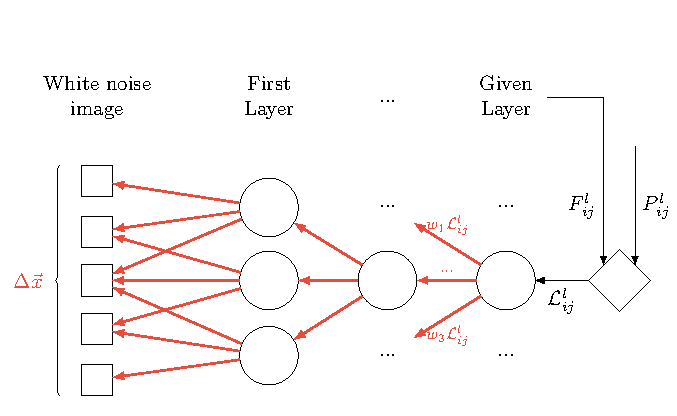
\includegraphics[width=\textwidth]{tkz/feature-reconstruction}
  \caption{
    Content reconstruction with standard backpropagation.
    The content loss $\mathcal{L}^l_c$ is numerically calculated for each neuron in a given layer $l$ from the content representation $F^l$ and $P^l$, resulting from the feed-forward pass of the white noise image $\vec{x}$ and the photograph $\vec{p}$ respectively.
    The calculated loss is backpropagated through the whole network until it reaches the first layer.
    The gradients $\Delta \vec{x}$ for adjusting the white noise $\vec{x}$ are calculated in the same way as if the input layer is a CNN layer.
  }
  \label{fig:system:method:feature-reconstruction}
\end{figure}

\paragraph{Style reconstruction}
Similarly, starting from a random white noise image $\vec{x}$, we will transform it to that it matches the style representation of an original artwork $\vec{a}$ in a number of CNN layers.
So, let $A^l$ and $G^l$ be the style representations of the original artwork $\vec{a}$ and the generated image $\vec{x}$, respectively, in layer $l$, we define the error as the mean-squared distance between the two representations:

\begin{equation}
  E_l =
  \frac{1}{4 N^2_l M^2_L} \sum_{i,j} (G^l_{ij} - A^l_{ij})^2
\end{equation}

Note this is not the loss function, since, unlike content representation, style representation is defined by the feature correlations $\{G^1, G^2, \dots, G^L\}$ in a number of layers.
Thus, we define the loss function to be minimized in style reconstruction as:

\begin{equation}
  \mathcal{L}_{style}(\vec{a}, \vec{x}) =
  \sum_{l \in L} w_l E_l
\end{equation}

Where $w_l$ are relative weights representing the contribution of each layer to the total loss $\mathcal{L}_{s}$.
Now, to obtain the gradients that will correct the white noise image $\vec{x}$ we must find the partial derivative of the loss function with respect to it.

\begin{equation}
  \Delta \vec{x} =
  \frac{\partial \mathcal{L}_{s}}{\partial \vec{x}}
\end{equation}

We can express the total loss in terms of the per-layer error as:

\begin{equation}
  \Delta \vec{x} =
  \frac{\partial \mathcal{L}_{s}}{\partial \vec{x}} =
  \frac{\partial \mathcal{L}_{s}(E_1, E_2, \dots, E_L)}{\partial \vec{x}}
\end{equation}

Which, applying the chain rule as described in \cite[Eq. 3.23]{Hairer2008}, can be rewritten as:

\begin{equation}
  \Delta \vec{x} =
  \sum_{l \in L} \Bigg(\frac{\partial \mathcal{L}_s}{\partial E_l} \frac{\partial E_l}{\partial \vec{x}}\Bigg) =
  \sum_{l \in L} \Bigg(w_l \frac{\partial E_l}{\partial \vec{x}}\Bigg)
\end{equation}

At this point, the only thing missing is calculating the derivative of the layer error $E^l$ with respect to the white noise image $\vec{x}$.
Finally, assuming $\vec{x}$ is the content representation $F^l$ in layer $l = 0$, we can generalize it for any layer $l$ by applying again the chain rule, which calculated for every neuron is expressed as:

\begin{equation}
  \frac{\partial E_l}{\partial F^l_{ij}} =
  \begin{cases}
    \frac{1}{N^2_l M^2_L} ((F^l)^T (G^l - A^l))_{ij} & \text{if } F^l_{ij} > 0 \\
    0                                                & \text{if } F^l_{ij} < 0
  \end{cases}
\end{equation}

Like in content representation, the gradients $\Delta \vec{x}$ can be obtained with standard error backpropagation to adjust the white noise $\vec{x}$ until its style representation matches that of $\vec{a}$ for the selected set of feature correlations $\{G^1, G^2, \dots, G^L\}$.

The results of separately reconstructing content and style can be seen in \autoref{sub:system:method:reconstructions}.
In content reconstruction, at the bottom, while visualizations generated from lower layers (a, b, c) preserve pixel fidelity compared with the input image, those generated from higher layers (d, e) lose pixel fidelity, since due to subsampling effects there is not enough information in the layer to exactly reconstruct the input image.
High-level content information is preserved in all cases, nonetheless, because the reconstruction process makes the neural activations produced by the input image and the generated one match, proof that feature maps in VGG-Network, trained in object recognition, precisely capture spatial information.
This is useful for the neural style algorithm to produce less hyperrealistic results when combining a photograph with an artwork.
In style reconstructions, at the top, visualizations have been generated with increasingly larger subsets of layers.
We observe how the texture transitions from colored noise (a), to just a cloud of colors (b), to clearer strokes (c, d), to bigger structures from the original artwork (d).
This is a consequence of the larger perceptive field of the filters in higher layers being able to capture bigger patterns that ultimately get transferred to the generated texture.
Being able to parametrize the texture is useful in the neural style algorithm to tweak how much detail of the style should be transferred, like in this example, where it should be small if we just want to transfer the characteristic style of strokes of Vincent van Gogh (b, c), or big if we also want shapes like the moon, clouds and the tower in \emph{The Starry Night}.

\begin{figure}[htb]
  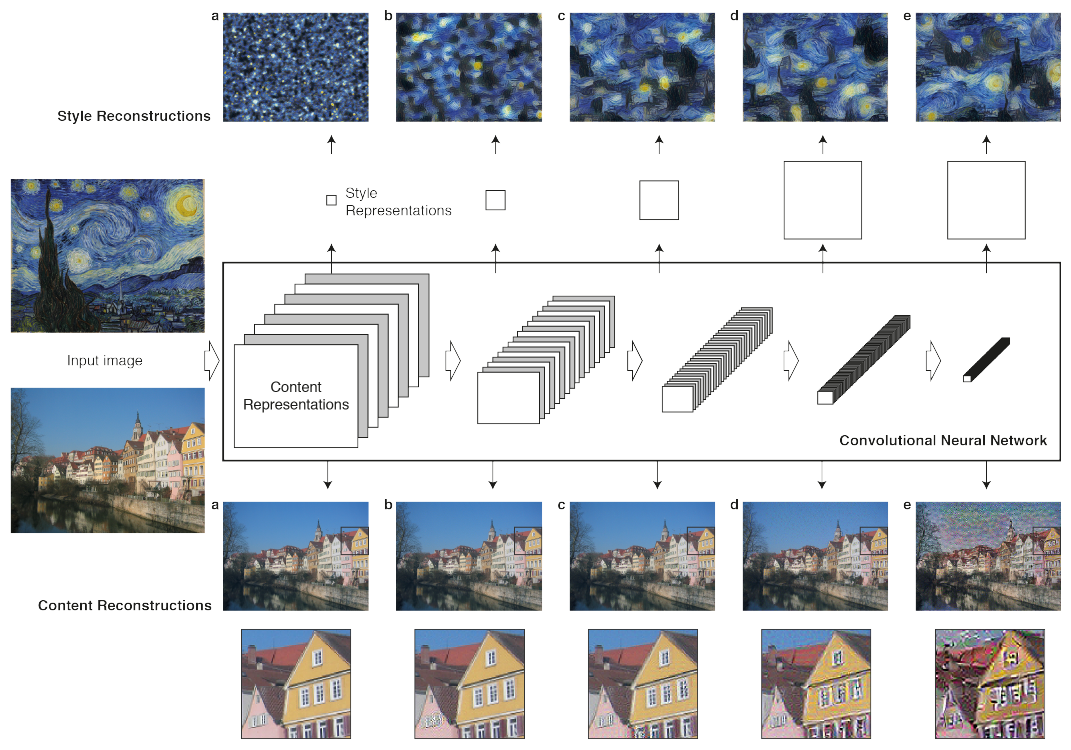
\includegraphics[width=\textwidth]{gfx/neural-style-cnn}
  \caption{
    Content and style reconstructions from an artwork and a photograph, respectively, using different feature maps from a CNN \cite{Gatys2015B}.
    As the input image gets processed by the CNN an increasing number of filter maps get produced in each layer.
    The totality of them for one layer are referred to in neural style as the content representation of the input image.
    At the bottom, content reconstructions of the photograph are generated at different stages of the VGG-Network from the following layers: ``conv1\_1'' (a), ``conv2\_1'' (b), ``conv3\_1'' (c), ``conv4\_1'' (d) and ``conv5\_1''.
    Style representations of an input image are built on top of content representations from a set of layers.
    At the top, style reconstructions of the artwork are generated using increasingly big subsets of layers: ``conv1\_1'' (a), ``conv1\_1'' and ``conv2\_1'' (b), ``conv1\_1'', ``conv2\_1'' and ``conv3\_1'' (c), ``conv1\_1'', ``conv2\_1'', ``conv3\_1'' and ``conv4\_1'' (d), ``conv1\_1'', ``conv2\_1'', ``conv3\_1'', ``conv4\_1'', and ``conv5\_1''.
    Including content representations from higher layers make the receptive field of style representations increase in size, and thus, the style reconstructions present larger local structures from the original artwork.
  }
  \label{sub:system:method:reconstructions}
\end{figure}


\subsection{Mixed Representation}
\label{sub:system:method:mixed-representation}

Having described how to separately reconstruct content and style from an original image it is straightforward to explain how the neural style algorithm is capable of simultaneously reconstructing both content and style from two different sources and producing the images in \autoref{sub:system:examples}.

Like in the previous cases, we want to find a new image $\vec{x}$ whose content representation and style representation matches at the same time the content representation of a photograph $\vec{p}$ in a given layer and the style representation of an artwork $\vec{a}$ in a set of layers.
Starting from a white noise image $\vec{x}$ the algorithm will simply need to minimize the following combined loss function:

\begin{equation}
  \mathcal{L}_{total}(\vec{p}, \vec{a}, \vec{x}) =
    \alpha \mathcal{L}_{content}(\vec{p}, \vec{x}) +
    \beta \mathcal{L}_{style}(\vec{a}, \vec{x})
\end{equation}

Where $\alpha/\beta$ is the ratio of emphasis of content over style, since content and style cannot be completely disentangled and a trade-off must be manually adjusted for each pair of source images.
The gradients $\Delta \vec{x}$, as before, are calculated with standard error propagation and are used to adjust the white noise image $\vec{x}$ until it reaches a compelling result.
The optimization process is one of huge dimensionality, taking into account the 144 million parameters in VGG-19 \cite{Simonyan2014}, and the unconstrained resolution of source images, and so \citeauthor{Gatys2015A} propose L-BFGS \cite{Zhu1994} as a suitable gradient optimization strategy.


% ------------------------------------------------------------------------------

\section{Results}
\label{sec:system:results}

\todo[inline]{Use my own results if enough time}

\citeauthor{Gatys2015B} presented in \cite{Gatys2015B} a series of results to showcase how each different hyperparameter affect the outcome of the algorithm as they vary.
As hinted while explaining the reconstruction process, the hyperparameters taken into account are three: 1) the ratio of emphasis on content over style $\alpha / \beta$, 2) the relative weights given to the CNN layers for style representation $\vec{w}_L$, and 3) which CNN layer is used for content representation.

\autoref{fig:system:results} shows results of some variations arranged in a grid where columns show variation in emphasis on content over style and rows variation of relative weights for style representation, having content representation fixed to CNN layer ``conv4\_2'' of the VGG-Network.
Although the style reconstruction method allows for arbitrary relative weights, \citeauthor{Gatys2015B} fixed on a simpler approach only using increasingly higher CNN layers and giving them equal relative weights.
In such configuration, relative weights for active CNN layers is set to $w_l = 1/n$, being $n$ the number of active layers, and to $w_l = 0$ for the rest.
Active CNN layers for style reconstruction per row: A) only ``conv1\_1'' ($w_l = 1$), B) ``conv1\_1'' and ``conv2\_1'' ($w_l = 1/2$), C) ``conv1\_1'', ``conv2\_1'' and ``conv3\_1'' ($w_l = 1/3$), D) ``conv1\_1'', ``conv2\_1'', ``conv3\_1'' and ``conv4\_1'' ($w_l = 1/4$), and finally E) ``conv1\_1'', ``conv2\_1'', ``conv3\_1'', ``conv4\_1'', and ``conv5\_1'' ($w_l = 1/5$).

\begin{figure}[!tb]
  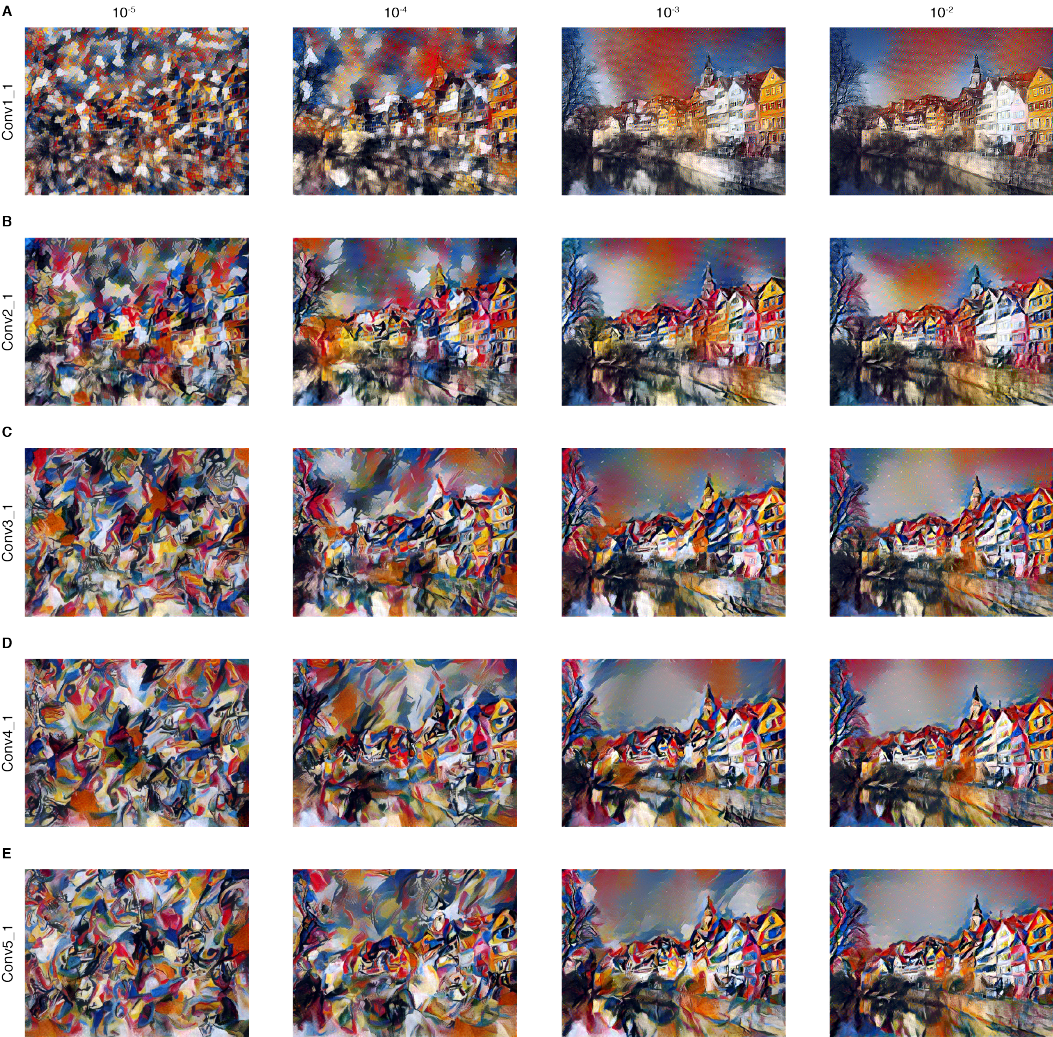
\includegraphics[width=\textwidth]{gfx/neural-style-results}
  \caption{
    Neural Style hyperparameter variation results of combining a photograph with the style of \emph{Composition VII} by Wassily Kandinsky.
    In the rows, from top to bottom, the increasing subset of CNN layers used for style representation, expressed with the higher layer used from VGG-Network (up to $conv\#\_1$).
    In the columns, from left to right, the increasing ratio $\alpha / \beta$ representing the emphasis on content over style.
    Including style features from higher layers of the network results in the style representation capturing bigger and more complex from the original artwork.
    Higher emphasis on content over style results in the synthesized image preserving more features of the original photograph.
  }
  \label{fig:system:results}
\end{figure}

Variations in emphasis on content over style show how increasing this ratio results on the features of the original photograph being preserved more faithfully.
If we look at \autoref{fig:system:results}~(A1), with a ratio of $10^{-5}$, very little is kept from the spatial information of the photograph and only some blue puffs representing the sky can be seen in the top region.
In \autoref{fig:system:results}~(A2), with a ratio of $10^{-4}$, the overall spatial arrangement of the photograph is already discernible, but, other than the closest building, the exact elements of the rest of the photograph are hard to tell.
Already in \autoref{fig:system:results}~(A3), with a ratio of $10^{-3}$, the buildings, river and tree are finally appreciable.
The exact spatial information remaining at the end is, however, dependent as well on the particular style representation chosen.

Now focusing on how the different style representations affect the outcome, we can see that including higher CNN layers makes the patterns increase in size and complexity.
The style representation captured ranges from showing little more than color puffs in \autoref{fig:system:results}~(A1), to similar shapes as seen in the original artwork in \autoref{fig:system:results}~(A5).
This makes sense if we think of CNNs trained in object recognition work.
Lower layers have small receptive fields and filters apply transformations that simply capture edges, corners or orientations.
On the other hand, higher layers have larger receptive fields due to subsampling and filters capture increasingly complex patterns such as shapes, text, or faces.

While Neural Style displays astounding capabilities for separation and mixing of style and content, compelling artistic results seem to be restricted to a particular region of hyperparameter values.
This region is not stationary as it varies from case to case depending on the photograph and artwork chosen and requiring careful fine-tuning of pixel fidelity (the chosen CNN layer for content representation), spatial information (the content-style ratio), and style representation complexity (the chosen CNN layers for style representation).


% ------------------------------------------------------------------------------

\section{Conclusion}
\label{sec:system:conclusion}

For the same reason \citeauthor{Gatys2015A} argues in \cite{Gatys2015A} about \citet{Portilla2000}'s approach not grasping the whole scope of natural textures which seems to have been solved I argue requiring human intervention for finding a set of hyperparameters in Neural Style that produce human compelling artistic composition is letting me think we are still far from understanding what describes art.

Neural Style astonishing results have caused quite a stir since they were presented in 2015.
In the next chapter, we will see how it has impacted the machine learning research community with derived work and promising further applications.

\todo[inline]{Complete discussion so that it connects with next chapter}

% All in all it is truly fascinating that a neural system, which is trained to perform one of the core computational tasks of biological vision, automatically learns image representations that allow the separation of image content from style. The explanation could be that when learning object recognition, the network has to become invariant to all image variation that preserves object identity. Representations that factorise the variation in the content of an image and the variation in its appearance would be extremely practical for this task. Thus, our ability to abstract content from style and therefore our ability to create and enjoy art might be primarily a preeminent signature of the powerful inference capabilities of our visual system.

% To understand our texture features better in the context of the original object recognition task of the network, we evaluated how well object identity can be linearly decoded from the texture features in different layers of the network. For each layer we computed the Gram-matrix representation of each image in the ImageNet training set [23] and trained a linear soft-max classifier to predict object identity. As we were not interested in optimising prediction performance, we did not use any data
% augmentation and trained and tested only on the 224×224 centre crop of the images. We computed the accuracy of these linear classifiers on the ImageNet validation set and compared them to the
% performance of the original VGG-19 network also evaluated on the 224 × 224 centre crops of the validation images.

% The analysis suggests that our texture representation continuously disentangles object identity in- formation (Fig. 4). Object identity can be decoded increasingly well over the layers. In fact, linear decoding from the final pooling layer performs almost as well as the original network, suggesting that our texture representation preserves almost all high-level information. At first sight this might appear surprising since the texture representation does not necessarily preserve the global structure of objects in non-texture images (Fig. 2, last column). However, we believe that this “inconsistency” is in fact to be expected and might provide an insight into how CNNs encode object identity. The convolutional representations in the network are shift-equivariant and the network’s task (object recognition) is agnostic to spatial information, thus we expect that object information can be read out independently from the spatial information in the feature maps. We show that this is indeed the case: a linear classifier on the Gram matrix of layer ‘pool5’ comes close to the performance of the full network (87.7% vs. 88.6% top 5 accuracy, Fig. 4)

% We envision that this will be useful for a wide range of experimen- tal studies concerning visual perception ranging from psychophysics over functional imaging to even electrophysiological neural recordings
% The style representations simply compute the correlations between different types of neurons in the network. Extracting correlations between neurons is a bio- logically plausible computation that is, for example, implemented by so-called complex cells in the primary visual system (V1)
% \cite{Adelson1985}

% !TEX root = ../thesis.tex

\chapter{Conclusion}
\label{chap:conclusion}

\cleanchapterquote{“Knowledge is just opinion that you trust enough to act upon.}{Orson Scott Card}{(Children of the Mind)}


% ------------------------------------------------------------------------------

In Chapter~\ref{chap:theory} we saw multi-layer feedforward neural networks are universal approximators.
A sufficiently big fully-connected network could, theoretically, solve arbitrarily complex problems.
However, limited computational resources and training datasets make them unpractical for real-world tasks.
Deep neural networks are used instead, as they learn increasingly abstract notions instead of raw inputs and require much fewer learnable parameters.
Traditionally, pattern recognition algorithms required domain features to be carefully modeled by experts with knowledge on the field, but Deep Learning allows us to train neural networks to carry out feature engineering automatically for us.

In Chapter~\ref{chap:context} we reviewed how the feature extraction capabilities of deep neural networks consistently granted them the top positions in object recognition challenges.
It is remarkable how well we understand how to make neural networks work for object recognition, as they now rival human performance in many aspects, compared to how little we know about how they reason once they are trained.
To help understanding this, recently-developed techniques try to visualize internal representations of deep neural networks and have produced very intriguing images with with potential artistic implications.

In Chapter~\ref{chap:system} we presented the Neural Style algorithm and how it managed to solve a long-standing problem in artistic rendering: the separation of style and content.
Whereas the algorithm can produce visually compelling compositions of style and content from two different source images, it requires fine-tuning on a per-case basis.
This make us believe Neural Style fails to grasp the notion of ``aesthetics'', which is another unsolved problem in artistic rendering, often studied in \emph{algorithmic aesthetics}.

In Chapter~\ref{chap:applications} we surveyed a number of methods for improved style transfer and several other image transformation tasks that also rely on extracting visually perceptive features.
They all presenting superior performance than the state of the art in their respective field.

The separation of style and content had been a very difficult problem to solve because it depends on human non-objective perception of what is style and what is content in an artwork.
Formulating notions of ``aesthetics'' is a similarly complex problem, since we cannot formally define it and totally builds upon human perception.

Capturing subjective opinions is being currently researched.
At the time of writing this thesis, the Beauty.AI's First International Beauty Contest Judged by an Artificial Intelligence Jury \cite{YouthLaboratories} has taken place already.
Their promoters, supported by Nvidia and Microsoft among others, aim for teaching machines estimate human attractiveness by looking at the human face, relying for this on human biased perception.

In the light of the increasing interest in distilling inherently subjective features that are impractically to model formally, we find the study of aesthetics a relevant matter with practical applications.
Therefore, we believe the aesthetics of images could be similarly distilled and used for further improving artistic rendering techniques.


% ------------------------------------------------------------------------------

\section{Future Work}
\label{sec:conclusion:future}

We propose further work on building an aesthetics-driven deep neural network for style transfer.
The system would consist of two sub-networks: one for image transformations, and another for quality estimation.
The image transformation network, once trained, would produce perceptually compelling images.
For training it, an aesthetic estimation network would rate the perceptual quality of the generated images and this would be used as the loss function.

The first challenge is finding how to quantify the perceptual quality of an image.
That is, to model an inherently human subjective notion.
For that we propose a convolutional neural network (CNN) that should be trained for estimating aesthetics based on human opinion.
The network could be either trained from scratch or from one pre-trained for object recognition, applying transfer learning techniques \cite{Pan2010}, which basically allows the network to adjust to a slightly different task or domain.

In order to train the aesthetics estimation network we must have a sufficiently large and diverse training dataset of image-rating pairs.
We imagine a crowdsourcing platform with which to collect ratings from humans on artistic compositions.
People would be presented with two artistic images and they should decide which two of them appeal most to them.
This is currently being done similarly in DeepArt.io's for the artistic Turing test (\url{https://turing.deepart.io/}).

The artistic images people would be rating could be composed of images from three sources: 1) a repository of classical paintings, 2) user-submitted style transfer creations, and 3) randomly-generated style transfer creations.
This last source would be generated from the repository of classical paintings, some repository of photographs, and randomly chosen style transfer hyperparameters.
Including them is of particular interesting since it will result in a more diverse, less biased artistic creations, and once ratings are collected, therefore, in a more representative training dataset for the aesthetic estimation network.

Important considerations to be taken when deploying the crowdsourcing initiative would be: acquiring a sufficiently large initial repository of images to rate, incentives to invite people to contribute, user interaction design to keep the contribution process simple, and, finally, potential partnerships with industry for having access to computation facilities in which to run the initiative.

The second challenge, once the aesthetic estimation network had been trained, is designing and training the image transformation network.
We have identified three plausible directions thus far.

Our first intuition is using a CNN whose very last layer is the Neural Style algorithm, as is.
The image transformation network in this case would learn how the Neural Style hyperparameters must be adjusted to produce a perceptually compelling composition given a pair of source images.

Likewise, our second approach is having the Neural Style hyperparameters fixed to some relatively good values.
In this case, the image transformation network would instead learn how to correct the source images so that when processed by Neural Style the result would be appealing.

We anticipate two main problems with the previous approaches.
First, Neural Style is computationally expensive, as it requires of a backpropagation pass to produce the images, and relying on it would terribly slow down the learning process.
And second, we suspect reusing Neural Style as a black box layer would limit the meaning of the internal representations.

To circumvent this, and inspired by \cite{Johnson2016}'s approach, we would completely disregard Neural Style in the image transformation network.
The network would learn how to maximize the perceived quality of the composition for a fixed style and a given photograph in a simple feedforward pass.
The question is still open to see if the network could learn how to apply general style transfer given two images.
We conjecture, however, that, by using the aesthetics estimation network as part of the loss function, it can be possible.

We are certain, such a system will not only pose a versatile tool for artistic rendering, it will also be of great relevance to the advance in neuroscience.
Giving researchers a new way to look into how the creative process occurs in the human brain and what are the patterns in nature that elicit the notion of beauty in our minds.

\begin{figure}[!b]
  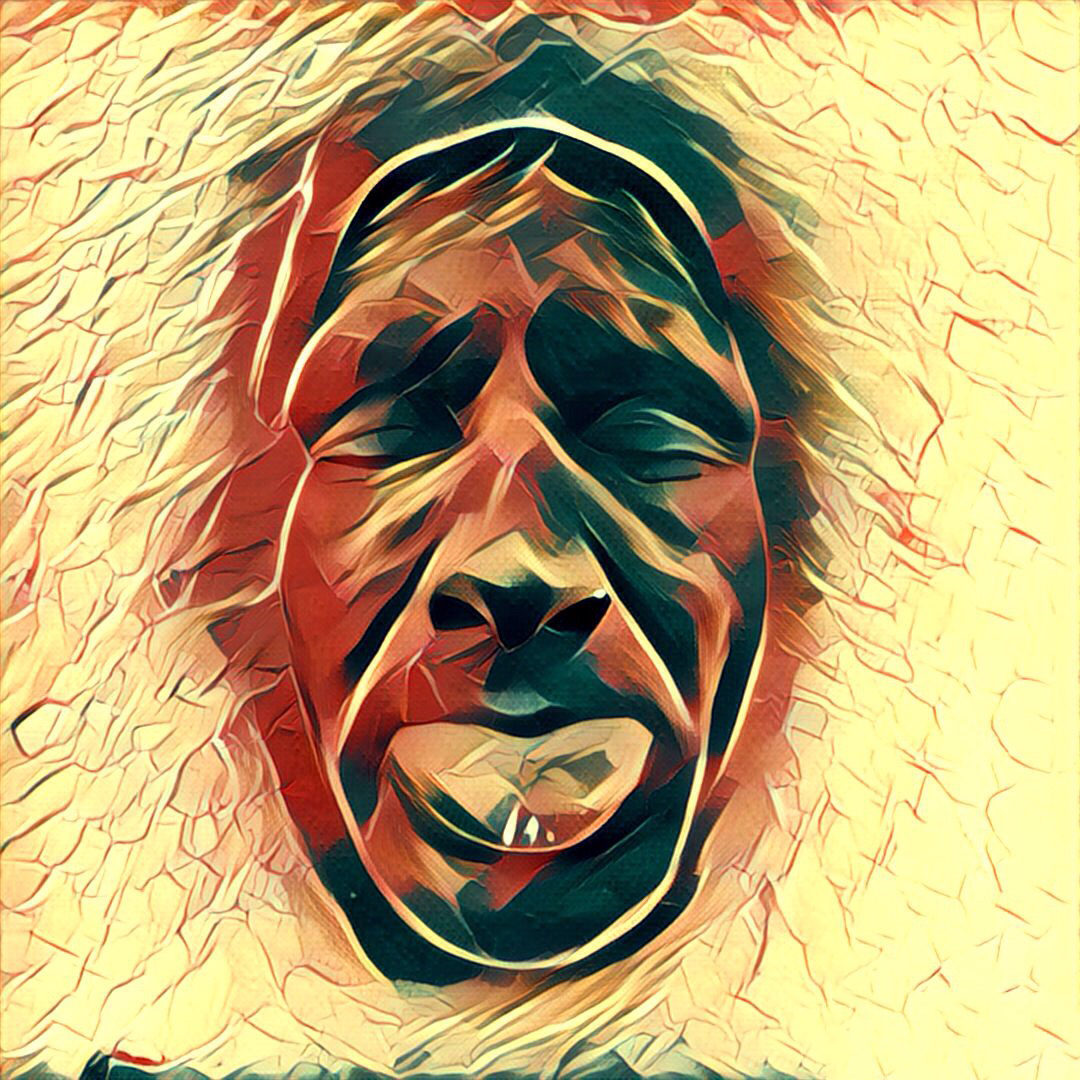
\includegraphics[width=\textwidth]{gfx/prisma}
\end{figure}

\cleardoublepage


% -- Back matter ---------------------------------------------------------------

{
	\setstretch{1.1}
	\renewcommand{\bibfont}{\normalfont\small}
	% \setlength{\biblabelsep}{0pt}
	\setlength{\bibitemsep}{0.5\baselineskip plus 0.5\baselineskip}
	\printbibliography[nottype=image]
	\printbibliography[heading=subbibliography,title={Images},type=image,prefixnumbers={!}]
}
\cleardoublepage

% !TEX root = ../thesis.tex
%
\pagestyle{empty}
\hfill
\vfill
\pdfbookmark[0]{Colophon}{Colophon}
\section*{Colophon}

This thesis was typeset with \LaTeXe.
It uses the \textit{Clean Thesis} style developed by Ricardo Langner.
The design of the \textit{Clean Thesis} style is inspired by user guide documents from Apple Inc.

Download the \textit{Clean Thesis} style at \url{http://cleanthesis.der-ric.de/}.

\cleardoublepage

% !TEX root = ../thesis.tex

\pdfbookmark[0]{Declaration}{Declaration}
\chapter*{Declaration}
\thispagestyle{empty}

I declare that I have completed my work solely and only with the help of the references mentioned above.

\bigskip
\noindent\textit{\thesisUniversityCity, \thesisDate}

\smallskip
\begin{flushright}
	\begin{minipage}{5cm}
		\rule{\textwidth}{1pt}
		\centering\thesisName
	\end{minipage}
\end{flushright}

\clearpage
\newpage
\mbox{}


% **************************************************
% End of Document CONTENT
% **************************************************

\end{document}
